\thispagestyle{plain}
\section{Single cell epigenomic landscape of\\human brain organoid development}
\markboth{Single cell epigenomic landscape of\\human brain organoid development}{}

\vspace{0.5cm}

Chapter 5 is a study entitled 'Single cell epigenomic landscape of human brain organoid development', which is currently \textit{in preparation}. I contributed major parts of the computational analyses for the presented scRNA-seq and scCut\&Tag data, including annotation, multi-modal integration, trajectory inference and differential expression analysis.

\vspace{1cm}

\noindent
{\large\textsc{Authors}}

\noindent
Fides Zenk\textsuperscript{1$*$}, 
Jonas Simon Fleck\textsuperscript{1$*$}, 
Sophie Martina Johanna Jansen\textsuperscript{1}, 
Bijan Kashanian\textsuperscript{1}, 
Benedikt Eisinger\textsuperscript{1}, 
Malgorzata Santel\textsuperscript{1}, 
J Gray Camp\textsuperscript{2,3}
Barbara Treutlein\textsuperscript{1}

\vspace{0.5cm}

\noindent
$\ast$ Equal contribution

\vspace{1cm}

\noindent
{\large\textsc{Affiliations}}

\noindent
\textsuperscript{1} Department of Biosystems Science and Engineering, ETH Zürich, Basel, Switzerland\\
\textsuperscript{2} University of Basel, Basel, Switzerland\\
\textsuperscript{3} Roche Institute for Translational Bioengineering (ITB), Roche Pharma Research and Early Development, Roche Innovation Center Basel, Switzerland

\vspace{1cm}

\noindent
{\large\textsc{Author contributions}}

\noindent
F.Z. generated organoids used in this study, with support from B.K. and M.S.. M.S. helped with iPS cell culture. F.Z generated all single-cell transcriptome and single-cell Cut\&Tag datasets with support from S.J.. F.Z. performed the drug-treatment, bulk Cut\&Tag and Western Blot experiments. F.Z. performed immunofluorescence experiments with support from B.E.. J.S.F. performed the analysis of the scRNA-seq/scATAC-seq developmental time course with support from F.Z.. J.S.F. analyzed the drug treatment scRNA-seq and bulk Cut\&Tag data with support from F.Z.. F.Z., B.T. and J.G.C. designed the study and F.Z., J.S.F., B.T. and J.G.C. wrote the manuscript.

\clearpage

\subsection{Abstract}

The cell type diversity of the human body originates from just one single totipotent cell. How the different cell types emerge from the same genomic sequence and how they maintain their identities throughout development is still an open question in biology. Epigenetic modifications that can direct the activity of genes and regulatory elements during development play an important role in the process of cell identity decisions.
Here, we explore how brain development and in particular, the differentiation of progenitor cells into different neuronal and glial cell types is regulated by epigenetic mechanisms. We use brain organoids to model the earliest events of cell fate acquisition in the developing brain and apply single-cell epigenetic profiling of histone modifications at various stages of brain organoid development. We use this data to reconstruct the epigenetic trajectory governing cell fate acquisition. We find that switching of epigenetic modifications can precede and predict the activation of important brain region-specific transcription factors. Further, we show that perturbation of histone modifiers during neuroectoderm establishment disrupts fate decisions and leads to aberrant cell fate acquisition. In summary, we provide the first comprehensive single-cell atlas of histone modifications during human brain organoid development, which will serve as a reference to understand early fate decisions but also neurodevelopmental diseases associated with chromatin regulators.


\subsection{Main}

During development and differentiation, cells undergo remarkable cell fate transitions starting from pluripotent cells and progenitors to give rise to all major cell types of the body. During these transitions, developmental plasticity becomes increasingly restricted until the cells stop dividing and acquire their terminal fate. Despite recent progress in epigenetics and reprogramming, the question of how cells acquire and maintain their identity on a global scale is still elusive. 

\begin{figure}[b!]
    \centering
	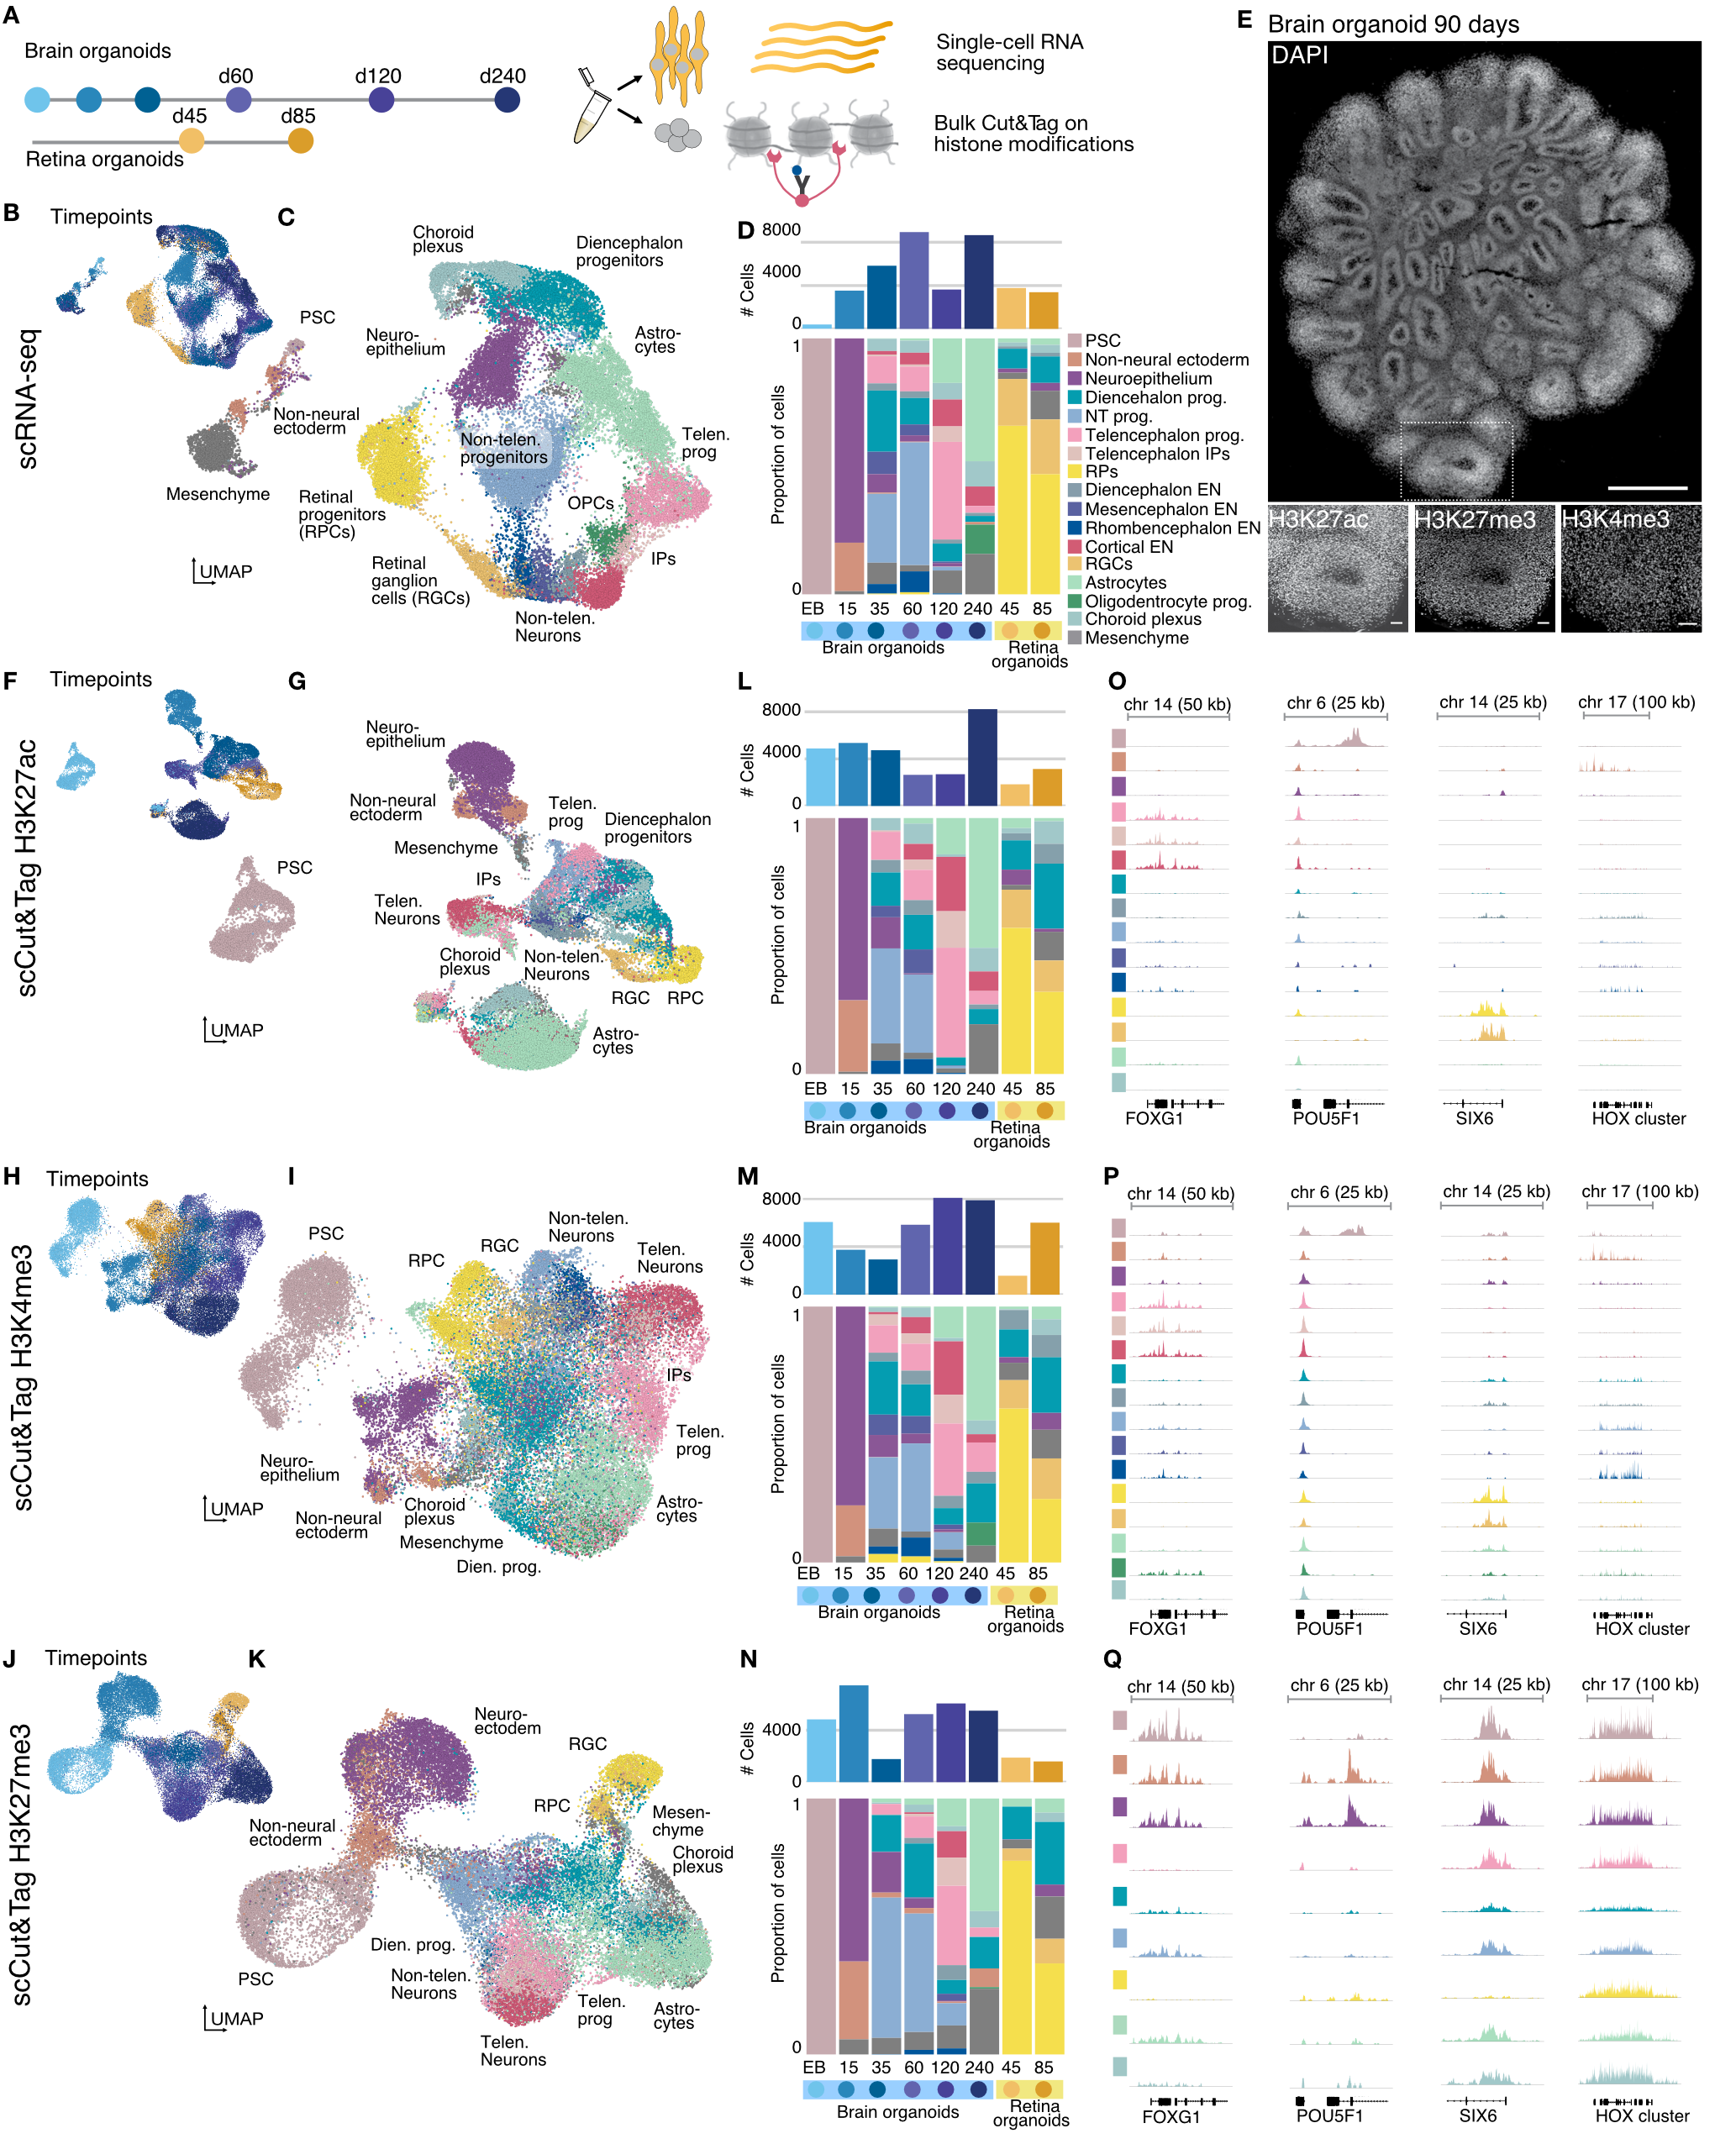
\includegraphics[width=\textwidth]{figures/cnt/Figure_1}
    \label{fig:cnt1}
\end{figure}

\begin{figure}[t!]
    \caption{\textbf{Single-cell epigenomic atlas of brain organoid development from pluripotency.}
    (A) Experimental outline. scCut\&Tag and scRNA-Seq were performed for different developmental timepoints during cerebral and retina organoid development. (B) UMAP embedding with cells colored based on developmental timepoint. (C) UMAP embedding with cells colored by celltype (IP - intermediate progenitor) (D) Bar-plot absolute cell number per timepoint (upper panel). Stacked bar plot of cell type distribution within each timepoint (lower panel) (EN - excitatory neuron, NT-non-telencephalon). (E) DAPI staining of an organoid at day 90, scale bar 1000 $\mu$m (upper panel). One ventricle of an organoid stained for H3K27ac, H3K27me3, H3K4me3, scale bar 100 $\mu$m (lower panel). (F, H, J) Same as (B) for H3K27ac, H3K4me3, H3K27me3, respectively. (G, I, K) Same as (C) for H3K27ac, H3K4me3, H3K27me3, respectively. (L, M, N) Same as (D) for H3K27ac, H3K4me3, H3K27me3, respectively. (O, P, Q) genome browser snapshots show the enrichment of the respective mark at four different marker genes (FOXG1-cortex, POU5F1-pluripotency, SIX6-retina, HOX-cluster-hindbrain and posterior parts of the body). Each signal track represents an annotated celltype.}
\end{figure}

\topparagraph{Single-cell epigenomic reconstruction of brain organoid development}
To address this question in the context of central nervous system development, we performed Cut\&Tag and mRNA-sequencing in single cells (scCut\&Tag and scRNA-seq) on a timecourse of human multi-region brain organoid development, modeling the cell fate transitions from induced pluripotent cells to terminally differentiated neurons. To cover all major lineages and cell types of the developing central nerveous system, we recorded three histone modifications and RNA expression at six developmental time points in brain organoids and two timepoints in retina organoids (Figure 5.1A and Figure S5.1A and B). During organoid development, cells transition from early pluripotent stages (embryoid body; day 5) to a stratified epithelium (neuroepithelium; day 15). From there, progenitors diversify and branch out to develop regional identities (telencephalon, diencephalon, non-telencephalon; day 35 and 60) (Figure 5.1B and C). Brain region-sepecific neurons start to develop from day 35 onward and later increase in abundance (Figure 5.1B, C and D). After day 120, astrocytes and oligodendrocyte precursor cells (OPCs) start to appear in the organoid, coinciding with the gliogenic switch during the second trimester of human embryonic development (Figure 5.1B, C and D) (\cite{rowitch_developmental_2010}). 

Having characterized the cell type and brain regional diversity of the developing organoids we asked how epigenetic changes on chromatin would contribute to fate decisions within the organoids. We first investigated the global distribution of H3K27ac, H3K27me3 and H3K4me3 by immunofluorescence at 90 days of organoid development. We found no major differences during the differentiation from the progenitor (localized at the center of the ventricles) to the neuron stage (localized on the outside of the ventricle) (Figure 5.1E). We then recorded the genome-wide distribution of H3K27ac, H3K27me3 and H3K4me3 by scCut\&Tag from cell suspensions matching scRNA-seq. We obtained high quality data from all experiments as reflected by the nucleosome pattern and the high average number of fragments (H3K4m3 - 2857, H3K27ac - 1723, H3K27me3 - 784) recovered from each cell (Figure S5.1C and D). Dimensionality reduction and embedding with UMAP (\cite{mcinnes_umap_2018}) revealed trajectories from early pluripotent cells over neuroectoderm to more differentiated cell states and brain region identities for each modality (Figure 5.1F-K).

To annotate cell types we first performed high-resolution Louvain clustering (\cite{blondel_fast_2008}) for each modality separately (RNA, H3K27ac, H3K27me3 and H3K4me3). Within high-resolution clusters we obtained on average 104k, 236k and 417k fragments (H3K27me3, H3K27ac and H3K4me3, respectively) and therefore increased the robustness of our analysis. We then annotated the high-resolution clusters of the scRNA-seq data using reference datasets (\cite{kanton_organoid_2019,fleck_inferring_2021}) and marker gene expression. Next, we matched scRNA-seq clusters with corresponding clusters from epigenomic modalities using minimum-cost, maximum-flow (MCMF) bipartite matching (\cite{stark_scim_2020}) based on correlation in case of activating histone marks (H3K27ac and H3K4me3) and anti-correlation in case of repressive mark H3K27me3 (Figure S5.2A and B). Based on these cluster-to-cluster matches we transferred annotated cell state labels from scRNA-seq to other modalities. We found that after label transfer, cell type and state distribution was similar between all modalities, supporting the accuracy of the integration (Figure 5.1L-M). In addition, we detected high enrichment of activating marks at known regulators of cell identity (e.g. FOXG1 in the telencephalic trajectory, POU5F1 in pluripotent stem cells, SIX6 in the retinal trajectory) (Figure 5.1O and P) and found the repressive mark H3K27me3 in cell states where the respective genes are not expressed (Figure 5.1Q). We were able to detect the same pattern of activating and repressive marks on genes marking brain region identities (SIX6, POU5F1, FOXG1, LHX5, NEUROD2, HOXB2) in single cells, which validates our annotation and label transfer (Figure S5.2C). Taken together, we here provide a comprehensive epigenomic atlas of cell type establishment and brain region diversification in organoids.

\begin{figure}[b!]
    \centering
	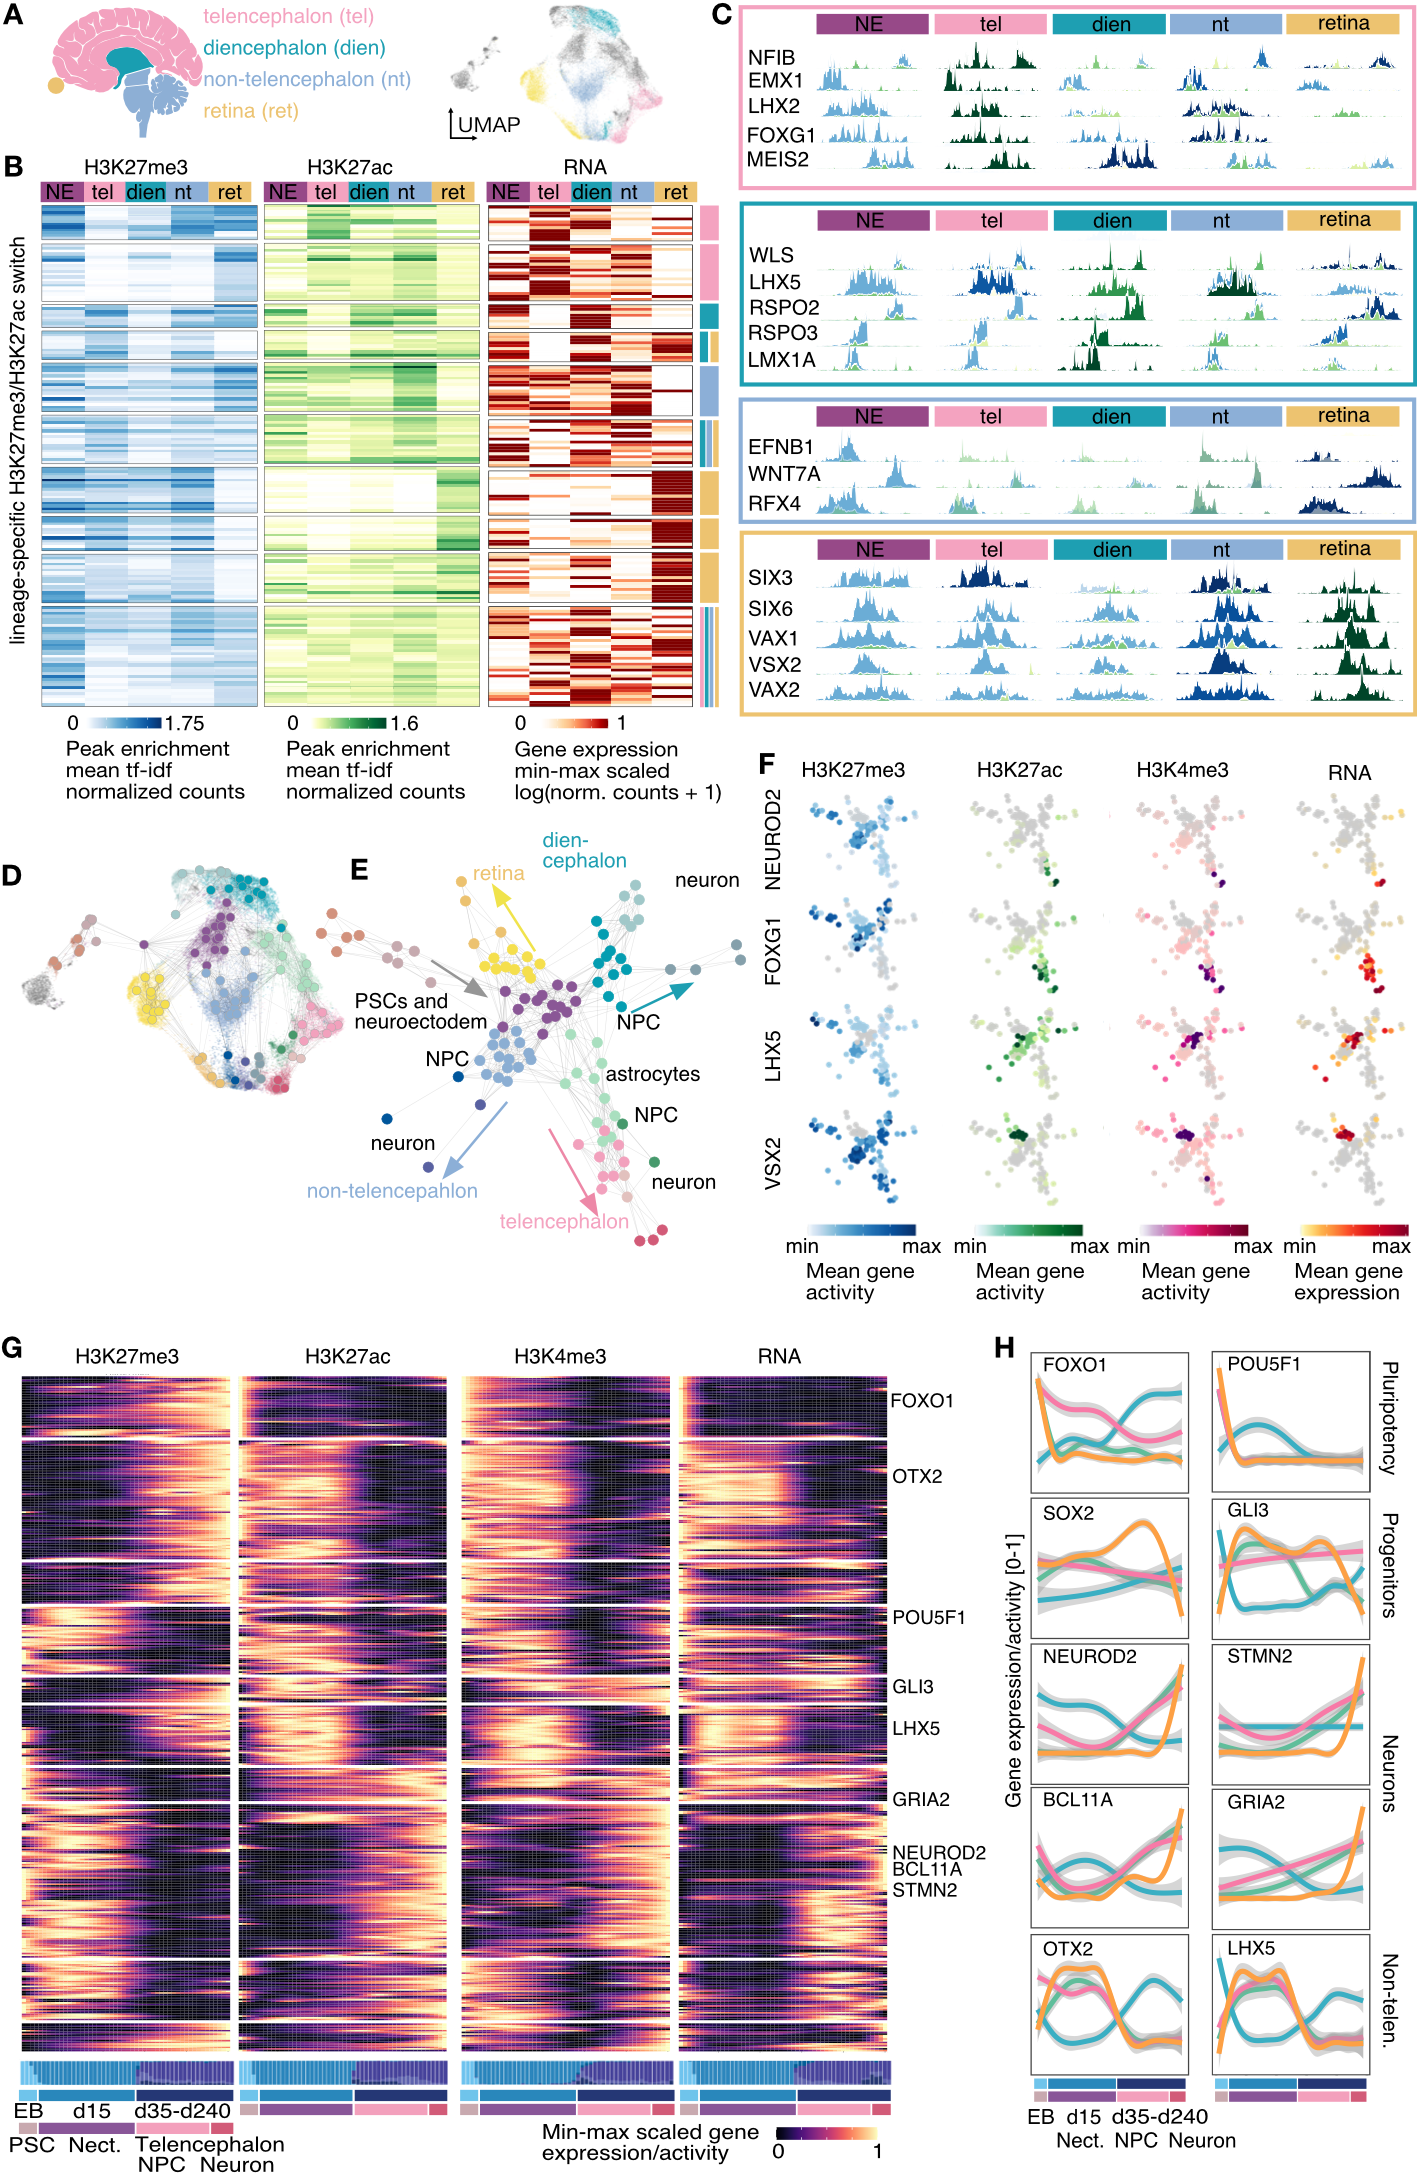
\includegraphics[width=0.9\textwidth]{figures/cnt/Figure_2}
    \label{fig:cnt2}
\end{figure}

\begin{figure}[t!]
    \caption{\textbf{Epigenomic switches and pseudotemporal dynamics during brain region diversification.}
    (A) Schematic of the human brain (left) and UMAP embedding (right) labelled with brain region identities. (B) Heatmap showing peak enrichment of lineage-specific peaks showing switching between H3K27me3 and H3K27ac marks. Expression of the closest gene is shown on the right. (C) Genomic tracks showing switching peaks close to lineage-specific genes. (D) UMAP representation and (E) graph layout of high-resolution clusters labelled by cell type. (F) Graph layout colored by expression and gene activities of all three chromatin marks for NEUROD2, FOXG1 (telencephalon), LHX5 (Non-telencephalon) and VSX2 (retina). (G) Heatmap showing expression and gene activity scores over the telencephalic neuron differentiation trajectory from pluripotency. Pseudotime was binned and genes were K-means clustered based on average expression/activity of all marks and RNA in all bins. (H) Line plots showing smoothed pseudotemporal expression and activities of selected examples from multiple K-means clusters.}
\end{figure}

\topparagraph{Epigenomic switches during regional diversification}
Regulatory elements can switch between a repressed state characterized by H3K27me3 enrichment and an active state marked by H3K27ac (\cite{allis_molecular_2016}). We observed that this is the case for elements in close proximity to many brain region-specific genes, i.e. genes repressed in early developmental stages and active in neurons of a given brain region. To characterize these region-specific switches more systematically, we first grouped all progenitors and neurons in our dataset based on regional identities (Figure 5.2A; telencephalon, non-telencephalon, diencephalon, retina). Next, we assessed regional specificity of peaks by performing differential enrichment analysis. We performed GREAT enrichment analysis (\cite{mclean_great_2010}) on region-specific peaks and found that activating marks H3K27ac and H3K4me3 were enriched in proximity to genes with important regulatory function for the respective region (Figure S5.3). Conversely, region-specific H3K27me3 (repressive) peaks were enriched at diverse genes with little or unspecific functional enrichment. To locate peaks exhibiting a switching behavior upon regional diversification, we intersected region enriched H3K27ac peaks with H3K27me3 peaks showing regional depletion. This revealed a set of peaks that are predominantly repressed during the neuroepithelial stage and switch into an active state in individual regional trajectories (Figure 5.2B). This epigenetic activation was accompanied by region-specific expression of nearby genes (Figure 5.2B), many of which were important regulators of regional identity, such as FOXG1 (telencephalon), RSPO2/3 (diencephalon), WNT7A (non-forebrain) and VSX2 (retina)(Figure 5.2C). Altogether, our analysis indicates that chromatin modifications can induce and stabilize regional diversification events by activating the expression of cell fate regulators.


\topparagraph{Epigenetic activation precedes gene expression during neurogenesis}
We next examined how these chromatin switches change dynamically along the differentiation trajectory from pluripotent stem cells to regionalized neurons. To better visualize the branching of neuroepithelial cells into progenitors and neurons of different brain regions, we used CellRank (\cite{lange_cellrank_2022}) to compute terminal fate probabilities for each regional identity based on RNA expression. We summarized these probabilities for each high-resolution cluster and used them to construct a graph representation of the differentiation events (Figure 5.2D). A force-directed layout of this graph revealed the bifurcation of pluripotent cells into non-neural ectoderm and neuroectoderm, which then diversifies into regional branches (Figure 5.2E). By mapping information from matched high-resolution clusters of chromatin modalities (Figure S5.2B) onto this representation, we could visualize changes in chromatin modifications along the differentiation trajectories (Figure 5.2F). To assess dynamic chromatin changes on the level of genes, we computed activity scores for each gene by summarizing fragment counts for each chromatin modification over the gene body plus an extended promoter region. Visualizing these gene activities on the graph layout made it apparent that many lineage-specific transcription factors were broadly repressed by H3K27me3 outside their expression domain (Figure 5.2F). 
Loss of repression within the respective lineage was accompanied by a gain in activating histone modifications immediately upon regionalization (Figure 5.2F; NEUROD2, FOXG1), which appeared to precede the increase in RNA expression.

To interrogate these developmental changes at higher resolution, we next examined one individual trajectory in isolation. To this end, we extracted cells belonging to the telencephalic neuron trajectory from pluripotency (PSC, neuroectoderm/neuroepithelium, telencephalon progenitor/neuron) and ordered them along a pseudotime axis using RNA velocity in case of RNA (\cite{bergen_generalizing_2020}) and diffusion maps in case of chromatin marks (\cite{haghverdi_diffusion_2016}). In order to obtain an even timepoint distribution over pseudotime for all modalities, we sub-sampled cells before grouping them into 50 equally sized bins (Figure 5.2G). After binning, the distribtion of sampling timepoints was similar between modalities and correlated well with pseudotemporal progression. 

To explore the dynamics of gene activation and repression during differentiation, we clustered genes based on their mean gene activity and expression within pseudotime bins. This revealed three major groups of genes with different switching dynamics. The first group exhibited a major switch between pluripotency and neuroectoderm stages, the second one between neuroectoderm and neural progenitor cell stages and the third one between neural progenitors and neurons (Figure 5.2G). We observed that during development many neuronal genes lose H3K27me3 mediated repression before accumulating H3K27ac and H3K4me3 and ultimately starting RNA expression (Figure 5.2G and H; NEUROD6, BCL11A, STMN2). These results support a model in which chromatin can be primed with activating histone modifications directing the expression of target genes in the future. At the same time, we captured the silencing of non-neuronal genes when cells exit from pluripotency and transition to neuroepithelium. These genes become down-regulated and lose active histone modifications while gaining H3K27me3 at the neuroepithelium stage. At more differentiated stages, these genes can remain silenced in absence of H3K27me3 (Figure 5.2G and H; POU5F1).

\begin{figure}[b!]
    \centering
	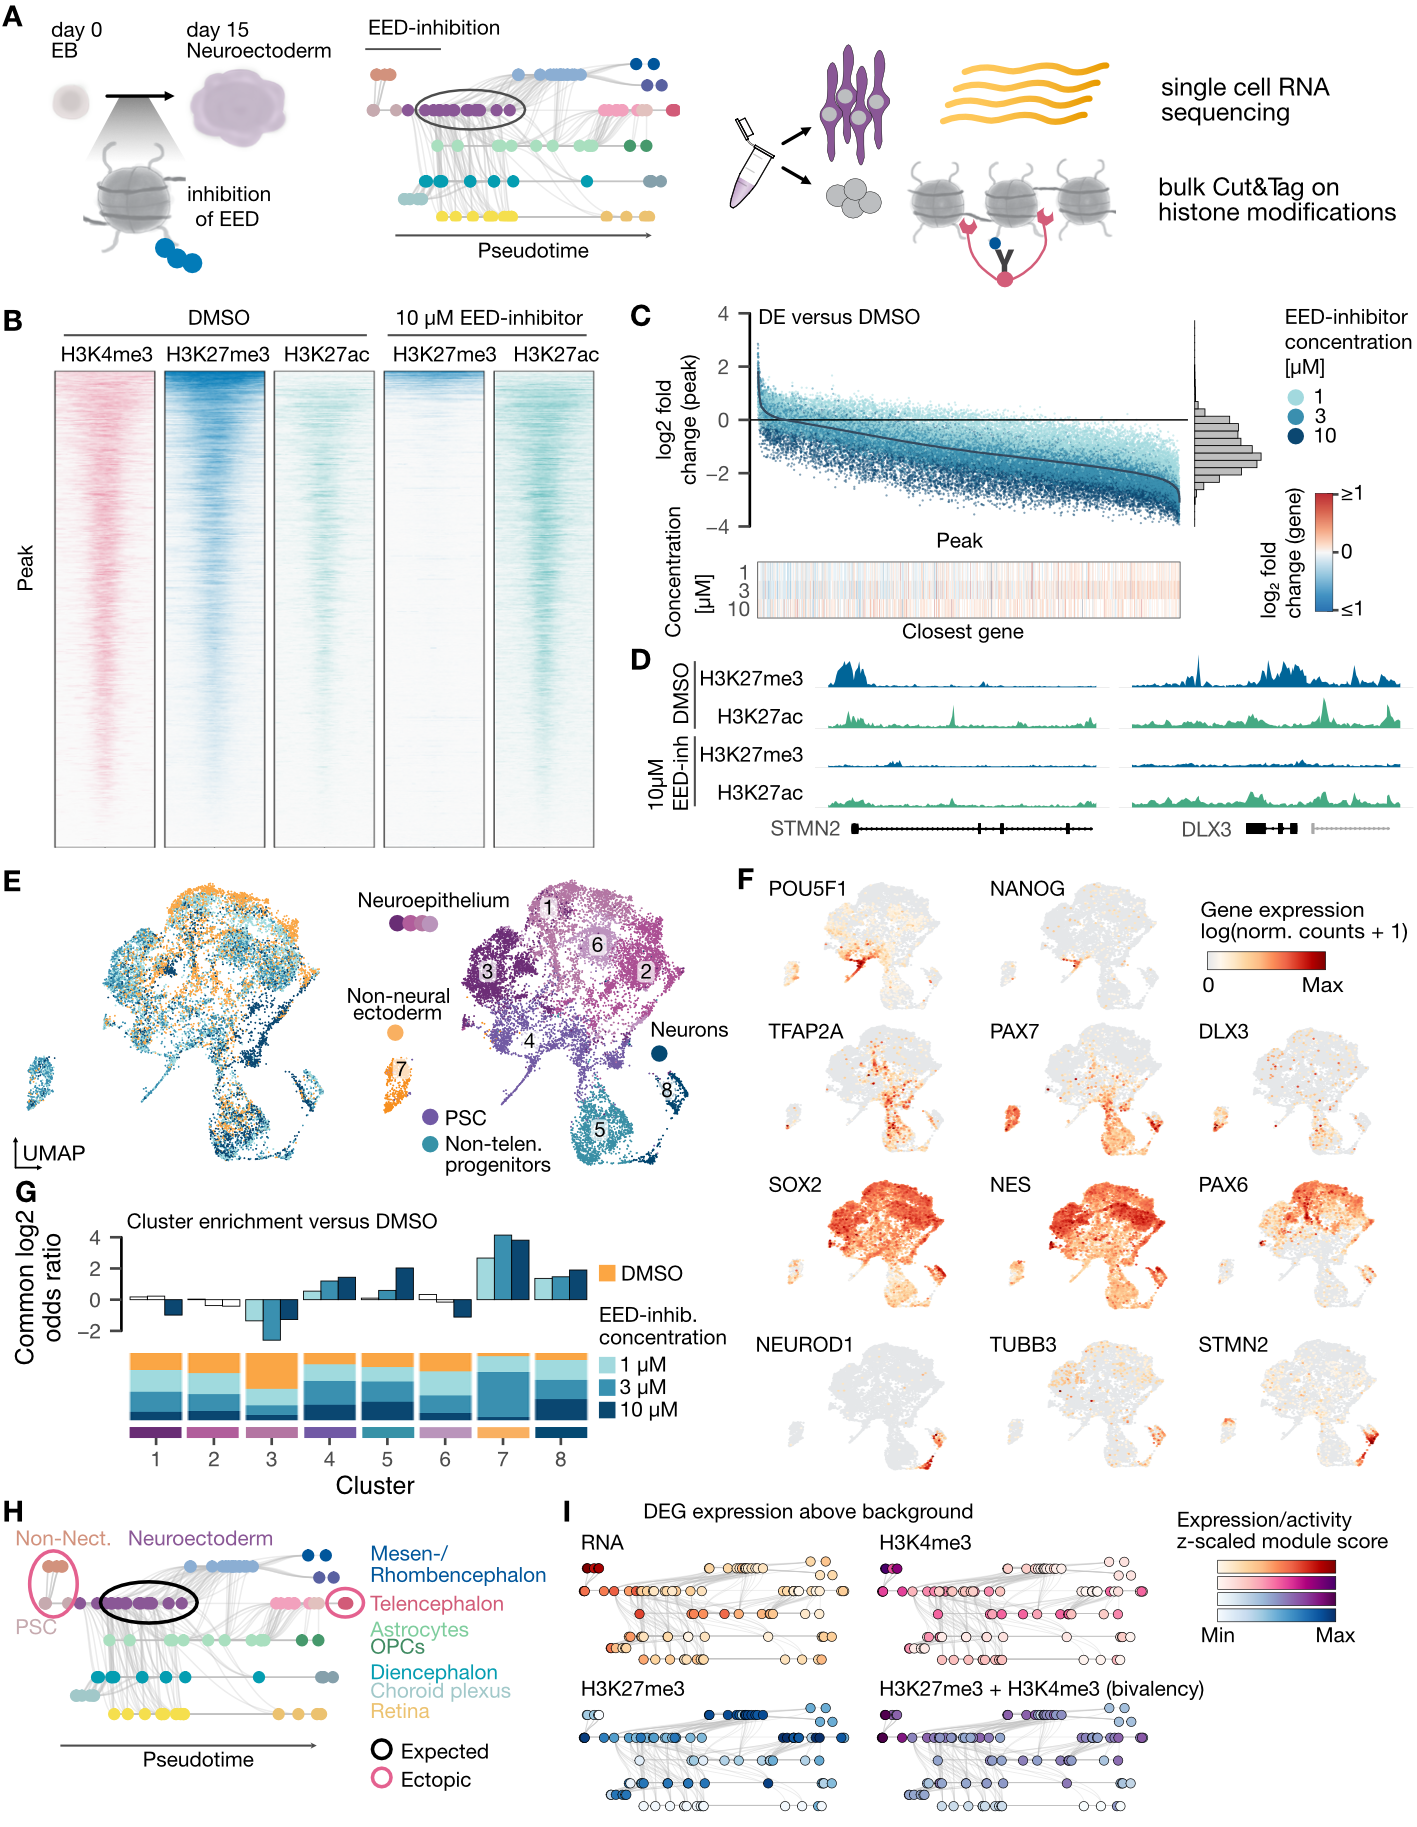
\includegraphics[width=0.9\textwidth]{figures/cnt/Figure_3}
    \label{fig:cnt2}
\end{figure}

\begin{figure}[t!]
    \caption{\textbf{Aberrant fate acquisition upon perturbation of EED.}
    (A) Schematic of the experiment. Organoids were treated with EED inhibitor from day 0 to day 15. During the neuroepithelium stage (day 15-18) organoids were profiled with scRNA-seq and bulk Cut\&Tag. (B) Heatmaps showing peak intensities from the bulk Cut\&Tag experiment for EED-inhibitor (10$\mu$M) and DMSO-treated organoids. Regions are ordered by H3K27me3 intensity. (C) Scatter plot showing log$_2$ fold change of peak intensities of organoids treated with different EED-inhibitor concentrations versus the DMSO control and histogram showing distribution of fold changes (top). Heatmap showing the log$_2$ fold change of expression of the closest gene from DE analysis in scRNA-seq data. (D) Genomic tracks showing bulk Cut\&Tag profiles for H3K27me3 and H3K27ac at genomic regions around STMN2 and DLX3. (E) UMAP embedding of the scRNA-seq data colored by treatment (left) and annotated louvain clusters (right). (F) UMAP embedding colored by expression of genes marking annotated populations. (G) Bar plot showing cluster enrichment of treated cells versus DMSO control (top) and distribution of treatments in clusters (bottom). Common odds ratio (height) and p-value (alpha) were obtained from a CMH-test stratified by sampling timepoint. (H) Tree representation of high-resolution clusters in the developmental timecourse, with the x-axis representing mean pseudotime. Cell populations commonly expected at day 15 (expected, black) and treatment-enriched populations (ectopic, red) are highlighted. (I) Tree representation colored by module scores (deviation above background) of DE gene expression and activity in the developmental timecourse.} 
\end{figure}


\topparagraph{Perturbation of histone modifiers causes aberrant fate acquisition}
The dynamic changes of histone modifications during regionalization and neurogenesis indicate that these epigenetic mechanisms play an important role in cell fate determination. To further investigate the role of histone modifications in shaping brain organoid development and cell differentiation, we chemically inhibited the writer complex of H3K27me3 (EED/PRC2) with A395 (\cite{he_eed_2017}) during the exit from pluripotency until the formation of the neuroepithelium (day 0-15). At the neuroepithelial stage (day 15-18) we profiled the organoids using scRNAseq and bulk Cut\&Tag (Figure 5.3A). Bulk Cut\&Tag measurements of histone modifications in EED-inhibitor and DMSO treated organoids showed an almost complete depletion of H3K27me3 marks upon treatment and an enrichment of H3K27ac marks at the same sites (Figure 5.3B). We quantified this depletion by computing the log$_2$ fold change of normalized H3K27me3 peak intensities versus DMSO control and found that repressive peaks were globally depleted in a concentration-dependent manner (Figure 5.3C). Next, we used the scRNA-seq data to quantify changes in gene expression upon treatment and extract a set of differentially expressed genes (DEGs). We observed a general up-regulation of gene expression, with genes in proximity to depleted peaks being more strongly affected. In the highest concentration of EED-inhibitor treatment, nearly all genes next to H3K27me3 peaks were significantly up-regulated (Figure 5.3B). As examples for this, we highlight the genes STMN2 and DLX3, around which repressive peaks are strongly depleted, resulting in an up-regulation of mRNA expression (Figure 5.3D).

We were curious how such drastic changes in gene expression would manifest on the level of cell states. To assess this, we integrated the scRNA-seq data between conditions, performed clustering and annotated the resulting populations (Figure 5.3E and F). As expected from this timepoint, we  observed a large neuroepithelial progenitor population (SOX2, NES, PAX6), but also pluripotent cells (POU5F1, NANOG) as well as populations of non-neural ectoderm (PAX7, DLX3) and neurons (STMN2, NEUROD1). Interestingly, despite the strong gene expression changes observed globally, both treated and control cells were present in all of these populations. However, differential abundance analysis revealed significant enrichment of treated cells in a number of clusters (Figure 5.3G). Most strongly and consistently affected were three ectopic clusters outside the main neuroepithelial population: non-neural ectoderm (cluster 7), pluripotent cells (cluster 4) and neurons (cluster 8). This indicates that treatment causes cells to increasingly adopt ectopic and off-target cell states (Figure 5.3H). To further investigate the relationship between dysregulated genes and cell state specification, we analyzed the expression and chromatin state of DEGs in the developmental atlas (Figure 5.3I). We found that during normal development, DEGs were predominantly repressed in the neuroepithelium and expressed in other populations, including pluripotent stem cells and non-neural ectodermal cells. Of note, DEGs also showed high bivalency (marked by both H3K4me3 and H3K27me3) in treatment-enriched cells states. Taken together, this analysis suggests that H3K27me3-mediated repression is required to stabilize neuroectoderm and neuroepithelium induction from pluripotency. Disruptions of H3K27me3 consequently leads to up-regulation of otherwise repressed or bivalent genes, causing cells to increasingly acquire aberrant and ectopic fates. 


\subsection{Discussion}
During early human brain development, gene expression has to be tightly coordinated to enable controlled differentiation into a multitude of defined cell types. Despite incredible progress in measurement technologies, it has so far remained challenging to interrogate the epigenetic mechanisms that shape these processes on a global scale and with single-cell resolution. 

Here we have addressed this challenge by measuring histone modifications at single-cell resolution in brain organoids, which model early human brain regionalization and cell type establishment \textit{in vitro}. Over a developmental organoid time course, we integrated scCut\&Tag profiles marking repressed and active chromatin states with RNA-expression data. Broadly, we found that chromatin modification profiles were highly specific for a given cell population. We identified region-specific regulatory chromatin regions and found that they controlled important regulators of cell fate. Such regulators were also often marked by epigenetic switches, which shift from repressive to active chromatin states at fate bifurcation events to prime gene expression. Generally, these observations indicate that chromatin modifiers play crucial roles in regional diversification events and stabilize cell fate commitment. This was further supported by perturbation of EED, which caused a global depletion of H3K27me3, an up-regulation of otherwise repressed genes and a strong tendency of cells to adopt off-target cell states. Inerestingly, a large fraction of cells still established neuroectoderm and neuroepithelium, even in the near complete absence of H3K27me3. This suggests that this is a default fate that cells assume in the absence of further inductive signals (\cite{argelaguet_multi-omics_2019,munoz-sanjuan_neural_2002}).  

Altogether, these results suggest that dynamic chromatin modifications are required to ensure robust cell fate acquisition and brain regionalization. Moreover, our developmental atlas of histone marks is the first of its kind and will serve as a reference to better understand the epigenomic landscape of human brain development.




\subsection{Methods}

\paragraph{Cell and organoid culture}
For culturing cells were grown on matrigel (Corning, \#354277) coated 6-well dishes in mTeSR Plus (StemCell Technologies, \#100-0276) supplemented with penicillin/streptomycin (P/S, 1:200, Gibco, \#15140122). To propagate the cells, they were dissociated with TryplE (Gibco, \#398 12605010) or EDTA in DPBS (final concentration 0.5mM) (Gibco, \#12605010) and kept on Rho-associated protein kinase (ROCK) inhibitor Y-27632 (final concentration 5 $\mu$M, StemCell Technologies, \#72302) for one day. Cells were stored in liquid nitrogen in mFreSR (StemCell Technologies, \#05855) and tested for mycoplasma (Venor GeM Classic, Minerva Biolabs) after each thawing cycle. 

To generate cerebral organoids, cells were grown to a confluency of around 50\% and dissociated with TryplE. 2000-3000 cells were aggregated in 96-well ultra low attachment plates (Corning, \#CLS7007) to form embryoid bodies (EBs). We followed an unguided protocol to obtain cerebral organoids5, with few modification. EBs were aggregated and cultured in mTeSR Plus and neural induction medium was added when the EBs had reached around 400-500 $\mu$m. Retinoic acid containing neural differentiation medium was only added from day 40 onward. Cerebral organoids were grown shaking in 6 cm dishes for up to 8 month.

To generate retinal organoids, we applied a protocol that allows the simultaneous aggregation of hundreds of embryoid bodies in agarose molds4. These are then transferred (1 week) to and later scraped off from 6-well plates (4 weeks), before they are transferred into differentiation medium.  
The use of human ESCs for the generation of cerebral organoids was approved by the ethics committee of northwest and central Switzerland (2019-01016) and the Swiss federal office of public health.

\paragraph{Drug treatment}
We used a pharmacological approach to inhibit chromatin modifiers in cerebral organoids. Specifically the H3K27-acetylase CBP/P3006 (A485, MedChemExpress, \#HY-107455) and the H3K27me3-reader EED7 (A395, MedChemExpress \#HY-101512, prevents allosteric activation of the PRC2 complex) were targeted. For A395 concentrations between 1-10 $\mu$M were tested and H3K27me3 was depleted in bulk experiments at 1 $\mu$M as shown by western blot. For A485 two concentrations (1 $\mu$M and 3 $\mu$M) were tested and H3K27ac, was depleted at 1 $\mu$M. 

CBP/P300 and EED were inhibited from day 0-15, by adding the inhibitor when seeding the EBs. This time window coincides with the formation of the neural epithelium. Following the medium was changed every 3 days adding a fresh dose of inhibitors. 
In a second experiment, CBP/P300 and EED were inhibited with 1 and 3 $\mu$M of the respective inhibitor from day 12-21, when brain regional markers start to be expressed in the organoid. 

To rule out cell line specific effects we treated two different cell lines (HOIK1 and WIBJ2) for the early timepoint and three (HOIK1, WIBJ2, WTC for 3 $\mu$M A395 and 1 $\mu$M A485) to five different cell lines (409b2- iCRISPR, B7, WTC, HOIK1 and WIBJ2 for DMSO, 1 $\mu$M A395 and 3 $\mu$M A485) for the late timepoint. We used single nucleotide polymorphisms (SNPs) to assign the cells bioinformatically to each cell line.

\paragraph{Preparation of single cell suspensions}
Cerebral organoids were generated in batches. In each batch five different stem cell lines (409b2- iCRISPR, B7, WTC, HOIK1 and WIBJ2) were used and dissociated together. The cell lines were later demultiplexed using single nucleotide polymorphisms (SNPs). For retinal organoids only B7 was used. We sampled all important developmental transitions from the pluripotent EB (day 5) and neuroepithelium (day 15) to neuronal differentiation in cerebral (day 35, 60, 120, 240) and  in retinal organoids (day 45 and 85). Organoids were cut into small pieces using a scalpel and thoroughly washed with HBSS buffer without Ca2+/Mg2+ (StemCell Technologies, \#37250) to remove debris. 

To obtain single cell suspension a papain-based neural dissociation kit (Miltenyi Biotec, 130-092-628) was used. In brief, 1900 $\mu$l of pre-warmed buffer X with 50 $\mu$l of Enzyme P were added to the organoids and incubated for 15 min at 37 °C. Subsequently, a mix of 20 $\mu$l buffer Y and 10 $\mu$l of DNase was added to each sample before tituration (10 times with a p1000 wide bore tip, 10 times with a p1000 wide bore tip). The samples were then incubated twice for another 10 min and titurated with a p1000 and p200 in between
 
At the end, the reaction was stopped with HBSS buffer without Ca2+/Mg2+ and the cells were passed through a 30 $\mu$m strainer. After an additional wash the cells were then stored in CryoStor CS10 (StemCell Technologies, Catalog \# 07930) or processed right away for further experiments. For all scCut\&Tag experiments, cells were kept from the same cell suspension to perform scRNA sequencing. Cell suspension usually exhibited viabilities between 80-95\%

\paragraph{Cloning and purification of Tn5}
Plasmids \#123461 (pA/G-MNase) and \#124601 (3XFlag-pA-Tn5-Fl) were ordered from Addgene. ProteinA and ProteinG were amplified using the primer pairs (FZ461\_ProtA\_rev,  
FZ462\_HindIII\_ProtA\_fw and FZ459\_EcoRI\_ProtG\_rev, FZ460\_ProtG\_fw) and fused by PCR (all primer sequences are in Table X, below). The ProteinA in the original vector (3XFlag-pA-Tn5-Fl)  was then replaced with the fusion product through EcoRI and HindIII restriction digest. 

The final plasmid was transformed into chemically competent Rosetta cells to express the protein. The bacteria were grown to OD600~0.4-0.6, expression was induced with 0.25 mM IPTG and the protein was expressed at 18 °C overnight. Cells were harvested and stored at -80 °C until further processing. The purification was performed on Chitin resin (New England Biolabs, \#S6651S) as described8, with small modifications. The cells were lysed using the Diagenode Bioraptor Plus at the high setting for 15 cycles 30 sec on/30 sec off.
After dialysis and concentration using Amicon Ultra-4 Centrifugal filters (Millipore, \#UFC803024) the protein was diluted to 50\% glycerol final and loaded with adapters before use: \\
FZ459\_EcoRI\_ProtG\_rev	gaattctttatcgtcatctacggctggcgtcaactcagacgcg \\
FZ460\_ProtG\_fw	aaaaagctaaacgatgctcaagcaccaaaaacaacttataaattagtcatcaacggg \\
FZ461\_ProtA\_rev	aatttataagttgtttttggtgcttgagcatcgtttagctttttagcttctgc \\
FZ462\_HindIII\_ProtA\_fw	ccaagcttaaaagatgacccaagccaaagtgctaacc \\
FZ444\_Tn5MErev	[phos]CTGTCTCTTATACACATCT \\
FZ445\_Tn5ME-A	TCGTCGGCAGCGTCAGATGTGTATAAGAGACAG \\
FZ445\_Tn5ME-B	GTCTCGTGGGCTCGGAGATGTGTATAAGAGACAG \\

\paragraph{Single cell Cut\&Tag}
Starting from 1.5-3 Mio cells, nuclei were isolated following the 10x Genomics CG000365 Demonstrated Protocol. The 0.1x buffer was used for all experiments, adjusting the final concentration of Digitonin to 0.01\% (Thermofisher, BN2006). In general we followed the bulk Cut\&Tag protocol with a few adjustments. 
After lysis the nuclei were directly transferred into scCut\&Tag wash buffer (20 mM HEPES [pH 7.5] (Jena Bioscience, \#CSS-511), 150 mM NaCl (Sigma Aldrich, \#S6546), 0.5 mM Spermidine (Sigma Aldrich, \#S0266), 1\% BSA (Miltenyi, \# 130-091-376), 1 mM DTT (Sigma Aldrich, \#10197777001), 5 mM sodium butyrate (Sigma Aldrich, \#303410), Roche Protease Inhibitor (Sigma Aldrich, \#11873580001)) and washed once for 3 min at 300 xg. The buffer was then supplemented with 2 mM of EDTA before the antibodies were added (see Table X for further details). The samples were then incubated on a rocking platform at 4 °C overnight. 

The next morning the cells were washed once and the secondary antibody was added to the suspension for 1 hr at 20 °C on a rocking platform or Eppendorf Thermomixer. The cells were then washed twice and transferred into scCut\&Tag med buffer (20 mM HEPES [pH 7.5] (Jena Bioscience, \#CSS-511), 300 mM NaCl (Sigma Aldrich, \#S6546), 0.5 mM Spermidine (Sigma Aldrich, \#S0266), 1\% BSA (Miltenyi, \# 130-091-376), 1 mM DTT (Sigma Aldrich, \#10197777001), 5 mM sodium butyrate (Sigma Aldrich, \#303410), Roche Protease Inhibitor (Sigma Aldrich, \#11873580001)) including 2 $\mu$g of homemade Tn5. The cells were incubated for 1 hr at 20 °C and then washed again twice with scCut\&Tag med buffer. To induce the cutting of the Tn5, 1 mM final MgCl2 (Sigma Aldrich, \#M1028) was added and the sample was incubated for 1 hr at 37 °C. After the incubation, the reaction was stopped with 15 mM EDTA final and the sample was filled to 600 $\mu$l with diluted nuclei buffer of the 10x Genomics scATAC kit v1.1 supplemented with 2\% BSA. The nuclei were filtered through a 40 $\mu$m Flowmi filter (Sigma Aldrich, \#BAH136800040) and washed with diluted nuclei buffer supplemented with 2\% BSA.

The final nuclei suspension quality controlled and counted with a Trypan Blue assay on the automated cell counter Countess (ThermoFisher). Finally 15-20k nuclei were loaded per experiment, in cases were fewer nuclei were recovered all were loaded. To run the Chromium Chip, 5 $\mu$l of cell suspension were mixed with 3 $\mu$l of PBS and 7 $\mu$l of ATAC buffer from the kit. 

Libraries were prepared following the manufacturer's instructions, except that 2 PCR cycles were added to the barcoding PCR and after 10 cycles of indexing PCR 5 $\mu$l of the library were used to determine the final number of cycles in a Roche LightCycler9. Usually sCut\&Tag libraries required 12-16 PCR cycles during the indexing. After SPRI select clean-up (Beckman Coulter, \#B23318) the libraries were quality controlled and sequenced following the 10x Genomics scATAC v1.1 sequencing recommendations. Usually 50-100 Mio reads per library were enough to cover the complexity. 

\paragraph{Bulk Cut\&Tag}
Starting with 0.1-1 Mio cells after dissociation, cells were transferred into Cut\&Tag wash buffer (20 mM HEPES [pH 7.5] (Jena Bioscience, \#CSS-511), 150 mM NaCl (Sigma Aldrich, \#S6546), 0.5 mM Spermidine (Sigma Aldrich, \#S0266), 5 mM sodium butyrate (Sigma Aldrich, \#303410), Roche Protease Inhibitor (Sigma Aldrich, \#11873580001)). Following 15 $\mu$l of BioMag ConcavalinA beads (Polysciences, \#86057-3) in binding buffer (20 mM HEPES (pH 7.5), 10 mM KCl, 1 mM CaCl2, 1 mM MnCl2) were added to the sample and incubated on the wheel for 15 min at RT. Subsequently the cells were collected on a magnet and lysed through the addition of Cut\&Tag wash buffer supplemented with 0.01\% Digitonin. Lysis was monitored under a microscope with Trypan Blue staining. After lysis was complete the nuclei were washed again with Cut\&Tag wash buffer. If possible all samples were split and H3 or another chromatin mark Cut\&Tag was performed on the same starting material, to be used as normalizer. The antibody was added together with 2 mM EDTA final and the sample was incubated on a rocking platform at 4 °C overnight.  
The samples were washed once with Cut\&Tag wash buffer and the secondary antibody was added to the reaction and incubated for 1 hr at 20 °C on a rocking platform. After two additional washes the Tn5 was added (1:100) in Cut\&Tag med buffer (20 mM HEPES [pH 7.5] (Jena Bioscience, \#CSS-511), 300 mM NaCl (Sigma Aldrich, \#S6546), 0.5 mM Spermidine (Sigma Aldrich, \#S0266), 5 mM sodium butyrate (Sigma Aldrich, \#303410), Roche Protease Inhibitor (Sigma Aldrich, \#11873580001)). Tn5 was allowed to bind for 1 hr at 20 °C on a rocking platform. After two additional washes the cutting was induced through addition of 1 mM MgCl2 in Cut\&Tag med buffer. After 1 hr at 37 °C the reaction was stopped by adding a final of 20 mM EDTA, 0.5\% SDS and 10 mg Proteinase K. The reaction was then incubated at 55 °C for 30 min and finally inactivated at 70 °C for 20 min.
 The DNA fragments were purified using the ChIP DNA Clean \& Concentrator kit (Zymo Research, \#D5205) for the elution from the columns 2 pg of Tn5-digested and purified lambda DNA (New England Biolabs, \# N3011S) were added to be used as spike-in normalizer for later analysis, when needed.

Purified fragments were indexed for 15 cycles (1 x 5 min at 58 °C, 1 x 5 min at 72 °C, 1 x	30 s at 98 °C, 14x 10 s at 98 °C, 30 s at 63 °C, 1 x 1 min at 72 °C, $\infty$ at 4 °C) using NEBNext HighFidelty 2x PCR Master Mix (New England Biolabs, M0541S) and Illumina i5 and i7 indeces9. The libraries were then purified using AmPure beads (Beckman Coulter, \#A63881), measured and quality controlled with Qubit DNA HS Assay (ThermoScientific, \#Q32854) and on the Tapestation (Agilent, \#5067-4626) and then sequenced (PE, 2x50 bp).

\paragraph{Hashing and single cell RNA-Seq}
Cells were either processed right after dissociation or recovered after cryostoring.  To recover the cells after cryostoring, the cryovials were incubated in a waterbath at 37 °C until only a small ice-piece was left inside the tube. The cells were then transferred into prewarmed DMEM/F-12 (Gibco, \#31330038) supplemented with 10\% FBS final (Merck, \#ES-009-B). After washing twice with DPBS (Gibco, \# 14190144) supplemented with 0.5\% BSA the cells were filtered with a 40 $\mu$m Flowmi filter and counted using the Trypan Blue assay on the automated cell counter Countess (ThermoFisher). Usually cell viability was around 80-95\%. At this point cells were further diluted to be processed in the 10x Genomics single cell RNA expression v3.1 assay following strictly the manufacturer's guidelines.

To generate single cell RNA expression libraries of the drug treatment we turned to cell hashing10 for better comparability of the samples. For hashing 100-300 k cells were resuspended in 50-100 $\mu$l of DPBS+0.5\% BSA. Following 5 $\mu$l of the Human TruStain FcX (Fc Receptor Blocking Solution, BioLegend, \#422302) were added to the sample and incubated for 10 min on ice.  Next, the 2 $\mu$l TotalSeq Cell hashing antibodies (BioLegend) were added to the cells and incubated for 30 min on ice with gentle agitation every 10 min. After incubation cells were washed twice with DBPS+0.5\% BSA. Depending on the starting amount the cells were resuspended in 20-40 $\mu$l DPBS+0.5\% BSA and counted. Following the cell suspensions were mixed and processed in the 10x Genomics single cell RNA expression v3.1 assay following strictly the manufacturer's guidelines with slight adjustments. A maximum of 20 k cells was targeted per experiment and HTO additive primer was added to the cDNA synthesis following the TotalSeq technical protocol (https://www.biolegend.com/en-us/protocols/totalseq-a-antibodies-and-cell-hashing-with-10x-single-cell-3-reagent-kit-v3-3-1-protocol). The generate gene expression and hashing libraries we followed the protocol CG000206 Chromium Next GEM SingleCell v3.1 Cell Surface Protein and sequenced according to the manufacturer's guidelines.

\paragraph{Western Blot}
Depending on the timepoint 1-3 organoids were directly collected into 50 $\mu$l Laemmli sample buffer and homogenized with an electric grinder (Fisherbrand 12-141-368). DNA was sheared by sonication in the Diagenode Bioraptor Plus (high setting for 15 cycles 30 sec on/30 sec off). Samples were subsequently run on SDS- PAGE and transferred to PVDF membrane using Wet-Blot. 2-10 $\mu$l of extract were loaded per lane. The ECL signal was recorded using iBright system (Invitrogen). The signal was compared to antibody stainings of loading controls (H3 and β-Catenin) and the membranes were quality controlled by Ponceau (Sigma Aldrich, \#P7170-1L) staining. See Table for details on the antibodies.

\paragraph{Immunostaining}
Organoids were fixed overnight in 4\% PFA. The next day, the organoids were washed three times for 5 min with DPBS and then transferred into 30\% sucrose in DPBS until they sank to the bottom of the tube. Following the organoids were transferred into cryomolds (Sakura, \#4565) and embedded in Tissue-Tek O.C.T. (Sakura, \#16-004004) on dry ice. The organoids were then sliced at the Cryostar NX70 (Thermo Scientific) into 20 $\mu$m thick slices at -17 °C. The slices were transferred to glass slides and washed with PBS. After a quick wash, antigen retrieval was performed for 20 min at 70 °C in 1x preheated HistoVT one (Nacalai, \#06380). Slides were washed 3 times for 5 min with PBS+0.2\% Tween and then transferred to blocking and permeabilization (PBS, 0.1\% Triton, 5\% Serum, 0.2\% Tween, 0.5\% BSA) for 1 hr. The antibodies were added in blocking solution overnight at 4 °C (see table for further details). The next day the slides were washed again 3 times for 5 min with PBS+0.2\% Tween and the secondary antibody was added in PBS supplemented with 2\% BSA and 0.2\% Tween for 2 hrs at room temperature. Last the slides were washed again 3 times for 5 min with PBS+0.2\% Tween adding DAPI to the last wash. The slides were then mounted in Prolong Glass Antifade and imaged at the Nikon Ti2 Spinning Disk or at the confocal Zeiss LSM980. 

\paragraph{Preprocessing scRNA-seq data}
To compute transcript count matrices sequencing reads were aligned to the human genome and transcriptome (hg38, provided by 10x Genomics) by running Cell Ranger (version 5.0.0)with default parameters. Count matrices were then preprocessed using the Seurat R package (version 3.2)(\cite{stuart_comprehensive_2019}). Cells were filtered by unique molecular identifier (UMI) counts, number of detected genes, and fraction of mitochondrial genes as follows:

\begin{itemize}
    \item \# UMIs > 2000 
    \item \# UMIs < 1.5 * 10\textsuperscript{5} 
    \item \# detected genes > 1000 
    \item fraction of mitochondrial reads < 0.2
\end{itemize}

Transcript counts were normalized by the total number of counts for that cell, multiplied by a scaling factor of 10,000 and subsequently natural-log transformed (NormalizeData()).

\paragraph{Preprocessing and clustering of scCut\&Tag data}
We aligned the sequencing reads to the human genome and transcriptome (hg38, provided by 10x Genomics) using Cell Ranger ATAC (version 1.2.0) with default parameters to obtain fragment files and peak calls. FThe fragment files and the peak count matrices were further preprocessed using Seurat (version 3.2)\cite{stuart_comprehensive_2019} and Signac (version 1.1)(\cite{stuart_multimodal_2020}). The following quality control metrics were computed using Signac: A transcription start site (TSS) enrichment score (TSSEnrichment()), nucleosome signal (NucleosomeSignal()), the percentage of reads in peaks, and the ratio of reads in genomic blacklist regions. Subsequently, cells with less than 200 (H3K27ac, H3K4me3) or 100 (H3K27me3) fragment counts were filtered out.

We then created a unified set of peaks from the union of peaks from all samples by merging overlapping and adjacent peaks. The unified set of peaks was requantified for each sample using the fragment file (FeatureMatrix()). Peak counts were normalized by term frequency-inverse document frequency (tf-idf) normalization using the Signac functions RunTFIDF(). Latent semantic indexing (LSI) was performed by running SVD (RunSVD()) on the tf-idf-normalized matrix. To visualize the data in 2D, Uniform Manifold Approximation and Projection (UMAP)(\cite{becht_dimensionality_2019}) was performed on LSI components 2-30. We then called high-resolution clusters using Louvain clustering in each group separately with the following resolutions to obtain similar cluster sizes:

\begin{itemize}
    \item EB: 2
    \item mid: 5
    \item late: 10
    \item 8 months: 5
    \item retina: 5
\end{itemize}


\paragraph{Demultiplexing}
We used demuxlet (\cite{kang_multiplexed_2018}) to demultiplex cells pooled from different stem cell lines. For B7 and 409B2-iCRISPR single nucleotide polymorphisms were called using bcftools based on DNA-seq data1,14 or downloaded from the HipSci website (HOIK1, WIBJ2) and the Allen Cell Atlas (WTC). All files were merged using bcftools and sites with the same genotypes in all samples were filtered out. Demuxlet was run with default settings. Cells with ambiguous or doublet assignments were removed from the data. Otherwise, the best singlet assignment was considered the lines' genotype.


\paragraph{Integration and annotation of scRNA-seq data}
First, we grouped the dataset into 5 groups depending on the sample of origin:  

\begin{enumerate}
    \item EB: 4 days old brain organoids in EB stage
    \item mid: 15 days old brain organoids in neuroectoderm stage
    \item late: 1-4 month old brain organoids
    \item 8 months: 8 month old brain organoids
    \item retina: 6 week \& 12 week old retina organoids
\end{enumerate}

Initial integration was based on mid and late groups. We computed the 2000 most variable features using the Seurat function FindVariableFeatures() and computed cell cycle scores using the Seurat function CellCycleScoring(). Subsequently the data was z-scaled, cell cycle scores were regressed out (ScaleData()) and Principal Component Analysis (PCA) was performed using the Seurat function RunPCA() based on variable features. We used the first 10 principal components (PCs) to integrate the different timepoints in the dataset using the Cluster Similarity Spectrum method (CSS)(\cite{he_css_2020}). The missing samples EB, retina and 8 months were then projected into CSS space using the css\_project() function. To obtain a two-dimensional representation of the data we performed Uniform Manifold Approximation and Projection (UMAP)(\cite{becht_dimensionality_2019}) using RunUMAP() with spread=0.8, min.dist=0.2 and otherwise default parameters.

To annotate the data, we first called high-resolution clusters using Louvain clustering in each group separately with the following resolutions to obtain similar cluster sizes:

\begin{itemize}
    \item EB: 1
    \item mid: 2
    \item late: 5
    \item 8 months: 2
    \item retina: 2
\end{itemize}

Clusters were annotated with cell types and regional identities using VoxHunt (\cite{fleck_resolving_2021}), comparison to reference datasets (\cite{kanton_organoid_2019,fleck_inferring_2021}) and marker expression.

\paragraph{Hashing}
Count matrices were generated with CITE-seq-Count (version 1.4.5 running under Python version 3.6.13) and intersected with transcript matrices from Cell Ranger. The hashtag counts were normalized with centered log-ratio (CLR) transformation. Doublets were filtered out using hashtag information. 

\paragraph{Calculation of gene activity scores}
To enable comparison of gene expression with chromatin modifications in the same feature space, we computed gene activity scores for each gene and chromatin modality. For this we used the Signac function GeneActivity() with default parameters. Fragment counts representing gene activities were subsequently log-normalized with a scaling factor of 10,000. 

\paragraph{Matching of scRNA and scCut\&Tag data}
To integrate cell populations between RNA and chromatin modalities, we matched high-resolution clusters based on correlation of gene expression with gene activity scores. For this, we performed minimum-cost maximum-flow (MCMF) bipartite matching between the modalities as described in \cite{stark_scim_2020} \\(https://github.com/ratschlab/scim). The function get\_cost\_knn\_graph() was used with \\knn\_k=10, null\_cost\_percentile=99 and capacity\_method='uniform'. As a distance metric (knn\_metric), we used the correlation distance provided by scipy (\cite{virtanen_scipy_2020}) for activating marks H3K27ac and H3K4me3 and the negative correlation distance for repressive mark H3K27me3. Unmatched clusters from either modality were matched based on maximum (or minimum) correlation. 


\paragraph{RNA velocity and inference of terminal fate probabilities}
To obtain count matrices for the spliced and unspliced transcriptome, we used kallisto (version 0.46.0)(\cite{bray_near-optimal_2016}) by running the command line tool loompy fromfastq  from the python package loompy (version 3.0.6)(https://linnarssonlab.org/loompy/). RNA velocity was subsequently calculated using scVelo (version 0.2.4)(\cite{bergen_generalizing_2020}) and further analyzed using scanpy (version 1.8.2)(\cite{wolf_scanpy_2018}). First, 2000 highly variable features were selected using the function scanpy.pp.highly\_variable\_genes(). Subsequently, moments were computed in CSS space using the function scvelo.pp.moments() with n\_neighbors=20. RNA velocity was calculated using the function scvelo.tl.velocity() with mode='stochastic' and a velocity graph was constructed using scvelo.tl.velocity\_graph() with default parameters. To order cells in the developmental trajectory, a root cell was chosen randomly from cells of the first time point (EB) and velocity pseudotime was computed with scvelo.tl.velocity\_pseudotime().  The obtained velocity pseudotime was further rank-transformed and divided by the total number of cells in the dataset. Based on the velocity pseudotime, we computed fate probabilities into the following manually annotated terminal cell states: Dorsal telencephalon neurons, diencephalon neurons, midbrain neurons, hindbrain neurons, retinal ganglion cells, astrocytes, oligodendrocyte progenitors, non-neural ectoderm and choroid plexus. For this, we used CellRank (version 1.3.0)(\cite{lange_cellrank_2022}). A transition matrix was constructed with a palantir kernel (PalantirKernel()) based on velocity pseudotime. Absorption probabilities for each of the predefined terminal states were computed using the GPCCA estimator.


\paragraph{Graph representation of the scRNA-seq data}
To better visualize the differentiation trajectories, we computed a graph representation based on the computed fate probabilities. Firest, we used PAGA to compute the connectivites between clusters (scvelo.tl.paga()) and summarized transition scores for each of the clusters. To find branch points at which the transition probabilities into different fates diverge, we then constructed a nearest-neighbor graph between the high-resolution clusters based on their transition scores (k=10). We further pruned the graph to only retain edges going forward in pseudotime, i.e. from a node with a lower velocity pseudotime to a node with a higher velocity pseudotime. Additionally, we removed edges connecting different regional trajectores. The resulting graph is directed with respect to pseudotemporal progression and represents a coarse-grained abstraction of the fate trajectory, connecting groups of cells with both similar transition probabilities to the different trajectories and high connectivities on the transcriptomic manifold. 


\paragraph{Trajectory reconstruction}
To reconstruct the telencephalic trajectory from pluripotency in higher resolution, we first extracted all cells annotated as EB, neuroepithelium, telencephalic progenitors and neurons. We next sought to compute a pseudotime describing the progression along this trajectory for all modalities separately. For all chromatin modalities, we used LSI components 2-10 to compute diffusion maps with the R package destiny (\cite{haghverdi_diffusion_2016}). Ranks along the first diffusion component were used as a pseudotemoral ordering. For RNA, we used the function scvelo.tl.velocity\_pseudotime() from scVelo (\cite{bergen_generalizing_2020}) to compute a pseudotime based on RNA velocity. To obtain a even distribution of timepoints for all modalities, we next subsamples the trajectory for each timepoint group to the lowest cell number in any modality but a minimum of 100. The subsamples trajectory was then stratified into 50 bins of equal cell number.

\paragraph{Preprocessing and integration of drug treatment scRNA-seq data}
The scRNA-seq data of A395 organoids was preprocessed analogous to the scRNA-seq data from the developmental timecourse. We then used Harmony (\cite{korsunsky_fast_2019}) with default parameters to integrate the different samples. Using the harmony integration, we performed louvain clustering with a resolution of 0.2 and annotated the clusters based on canonical marker gene expression.

\paragraph{Preprocessing of bulk Cut\&Tag data}
The fastq reads from the bulk Cut\&Tag experiment were aligned to the human genome (hg38) using bwa (\cite{li_fast_2009}). Next, normalized bigwig files were obtained using deeptools bamCoverage (\cite{ramirez_deeptools2_2016}) with --ignoreDuplicates, -bs 200 and --normalizeUsing RPKM. 

\paragraph{Differential peak analysis}
To obtain enrichment scores on the level of peaks, we summarized normalized bigwig files to the peaks from the developmental timecourse for each modality. Based on these peak intensities, we computed the log$_2$ fold change of treated versus control samples for each sample and concentration separately. The log$_2$ fold changes were then summarised by taking the mean for each concentration.

\paragraph{Differential gene expression analysis}
To assess the changes in gene expression upon treatment with A395, we performed differential expression (DE) analysis based using a logistic regression framework. To test for global DE while accounting for conpositional differences, we considered the louvain cluster label as a covariate in the model. We further accounted for sampling timepoint and sequencing depth (UMI count):

\[ Y_i \sim n\_UMI + timepoint + louvain\_cluster + treatment \]

We used the Seurat function FindMarkers() to perform the test for each condition separately and for all conditions combined. The resulting p-values were FDR-adjusted using the Benjamini-Hochberg method. We used a significance threshold of FDR < 0.01 and absolute log$_2$ fold change > 0.1.


\paragraph{Differential abundance analysis}
To test for compositional differences upon treatment with A395, we perfromed a Cochran-Mantel-Haenzel test stratified by sampling timepoint for each louvain cluster and concentration separately. The resulting p-value was FDR-corrested and a significance threshold of $10^-4$ was applied.








\clearpage

\subsection{Supplement}
\beginsupplement

\begin{figure}[h!]
    \centering
	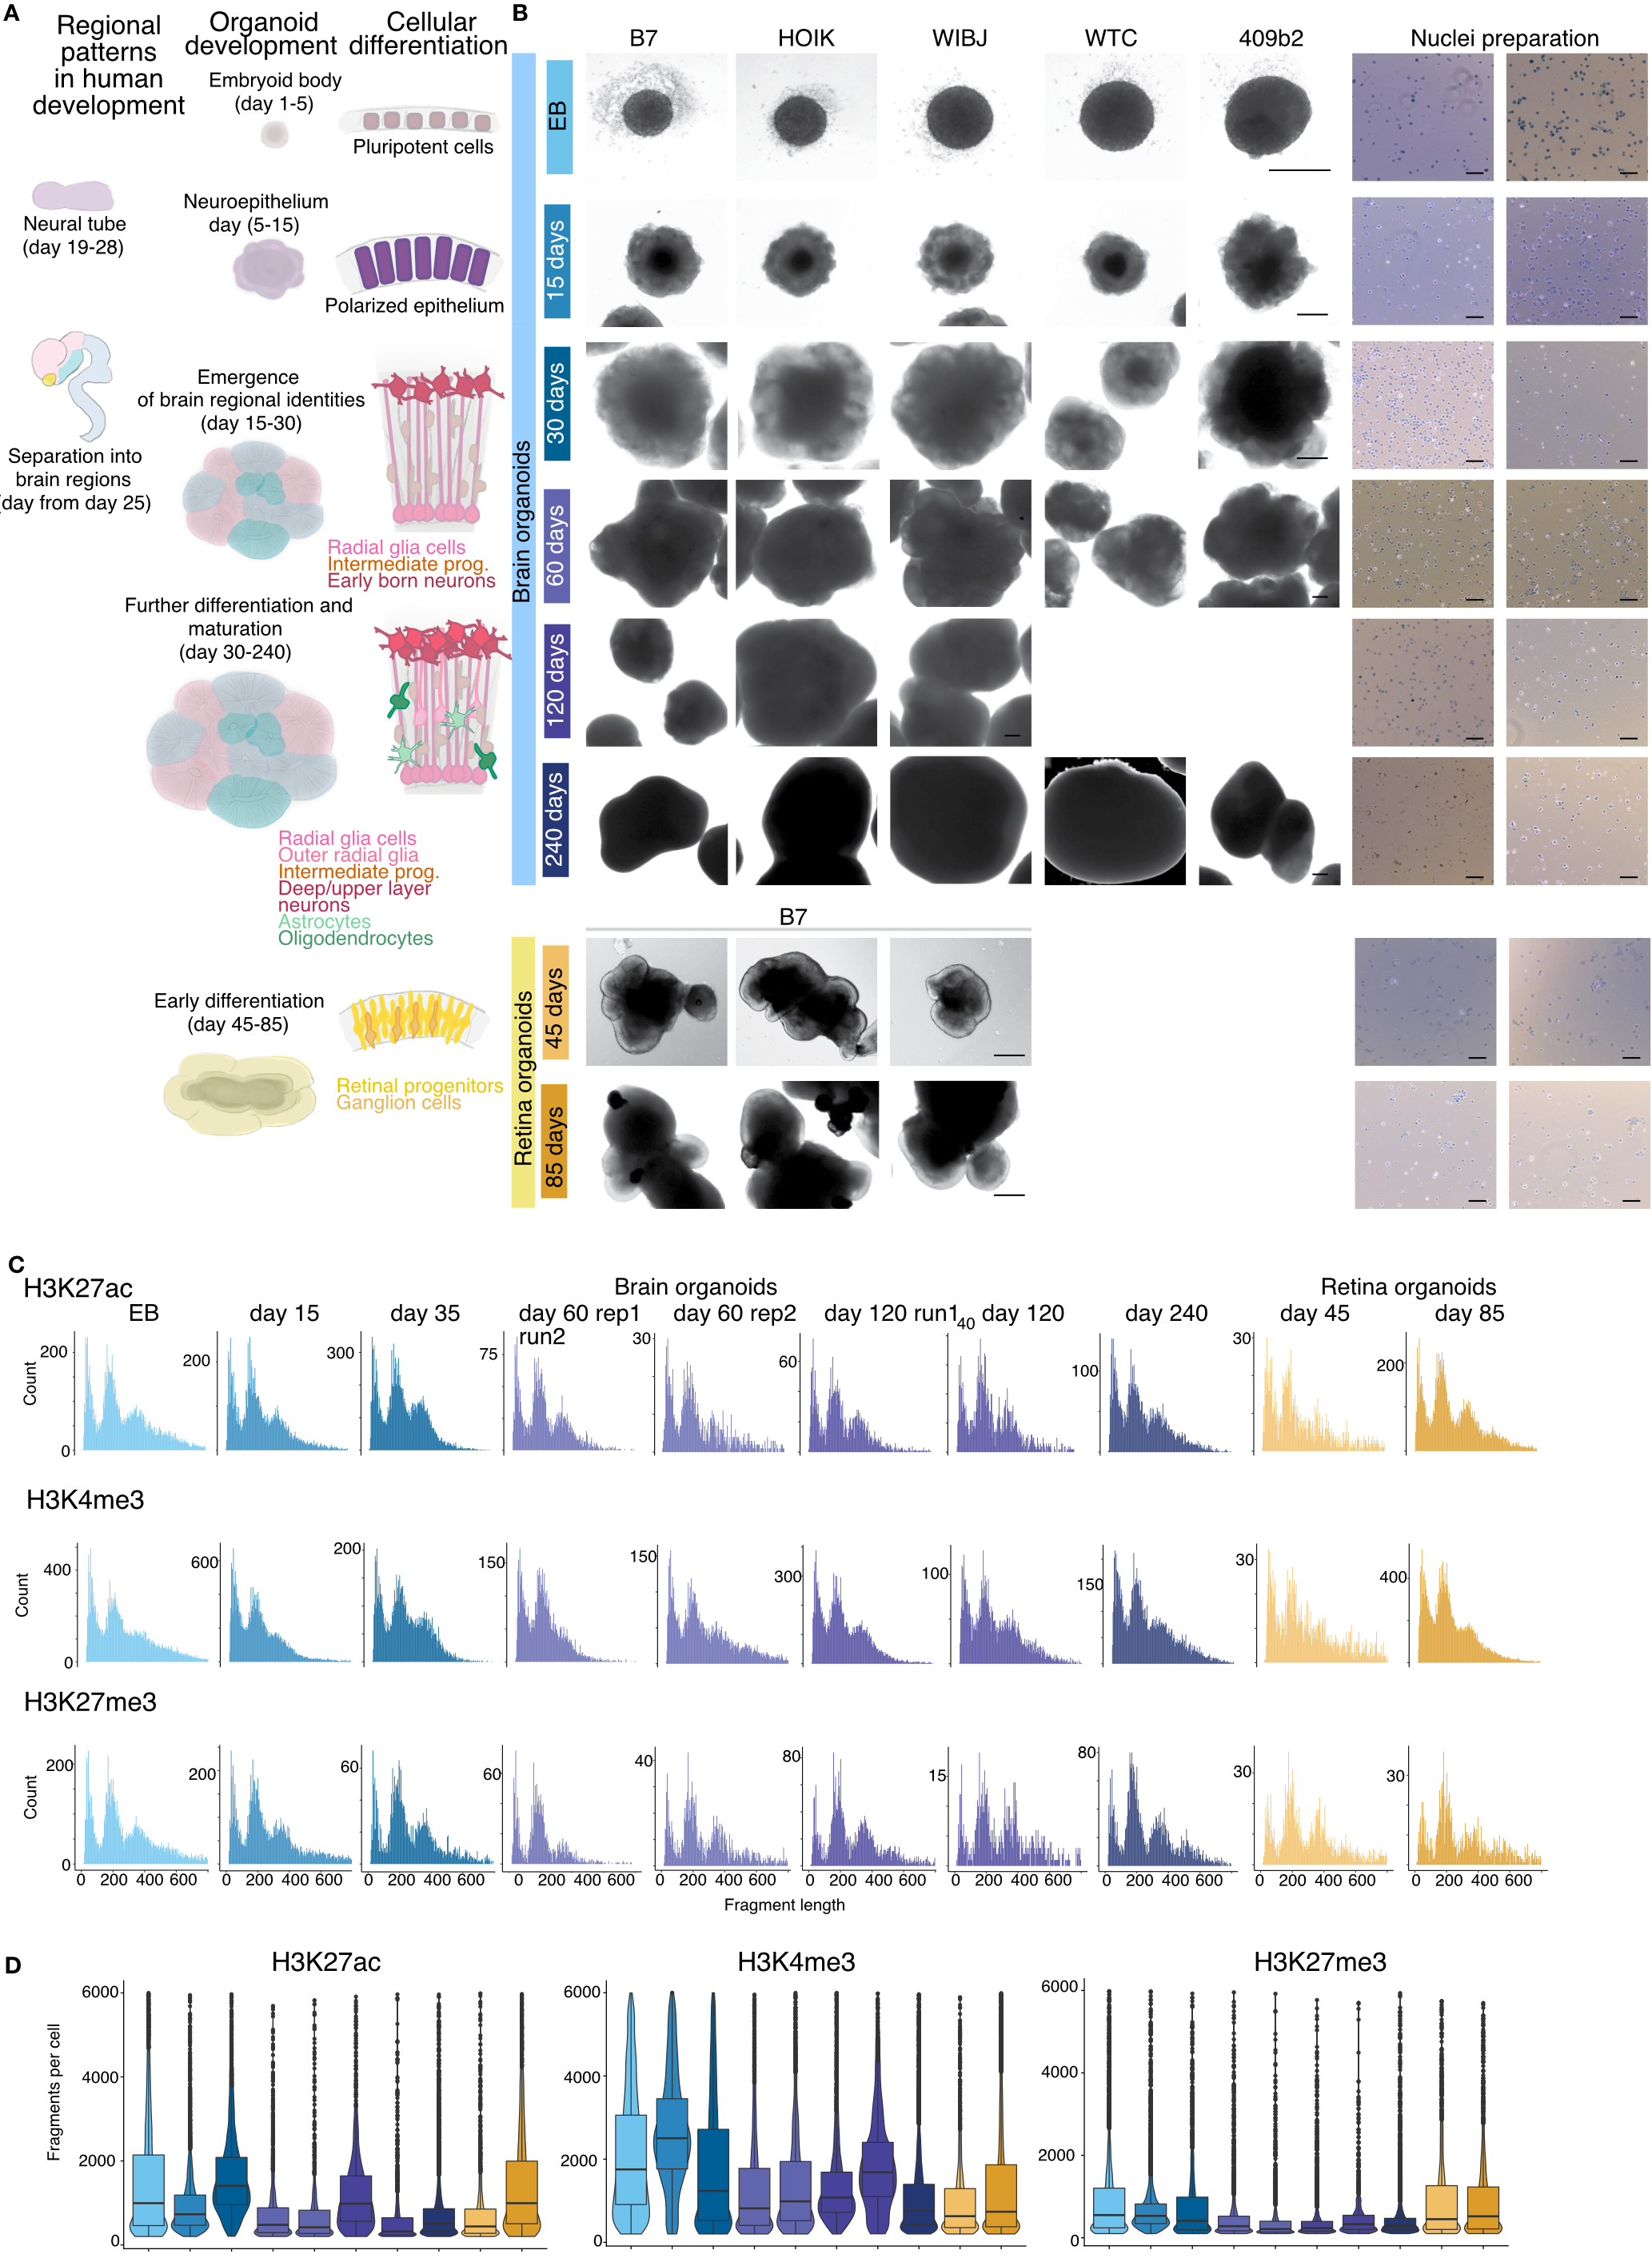
\includegraphics[width=0.9\textwidth]{figures/cnt/Figure_S1}
    \label{fig:regS1}
    \caption{\textbf{Quality control for epigenomic atlas of brain organoid development.}
    (A) Schematic of brain and retina organoid development in relation to early human brain development and emergence of cell type heterogeneity. (B) Brightfield images of organoids during development. (C) Histograms showing fragment length distribution for all samples and modalities. (D) Violin plots showing the distribution of detected fragments per cell for each timepoint and chromatin modality.}
\end{figure}


\begin{figure}[h!]
    \centering
	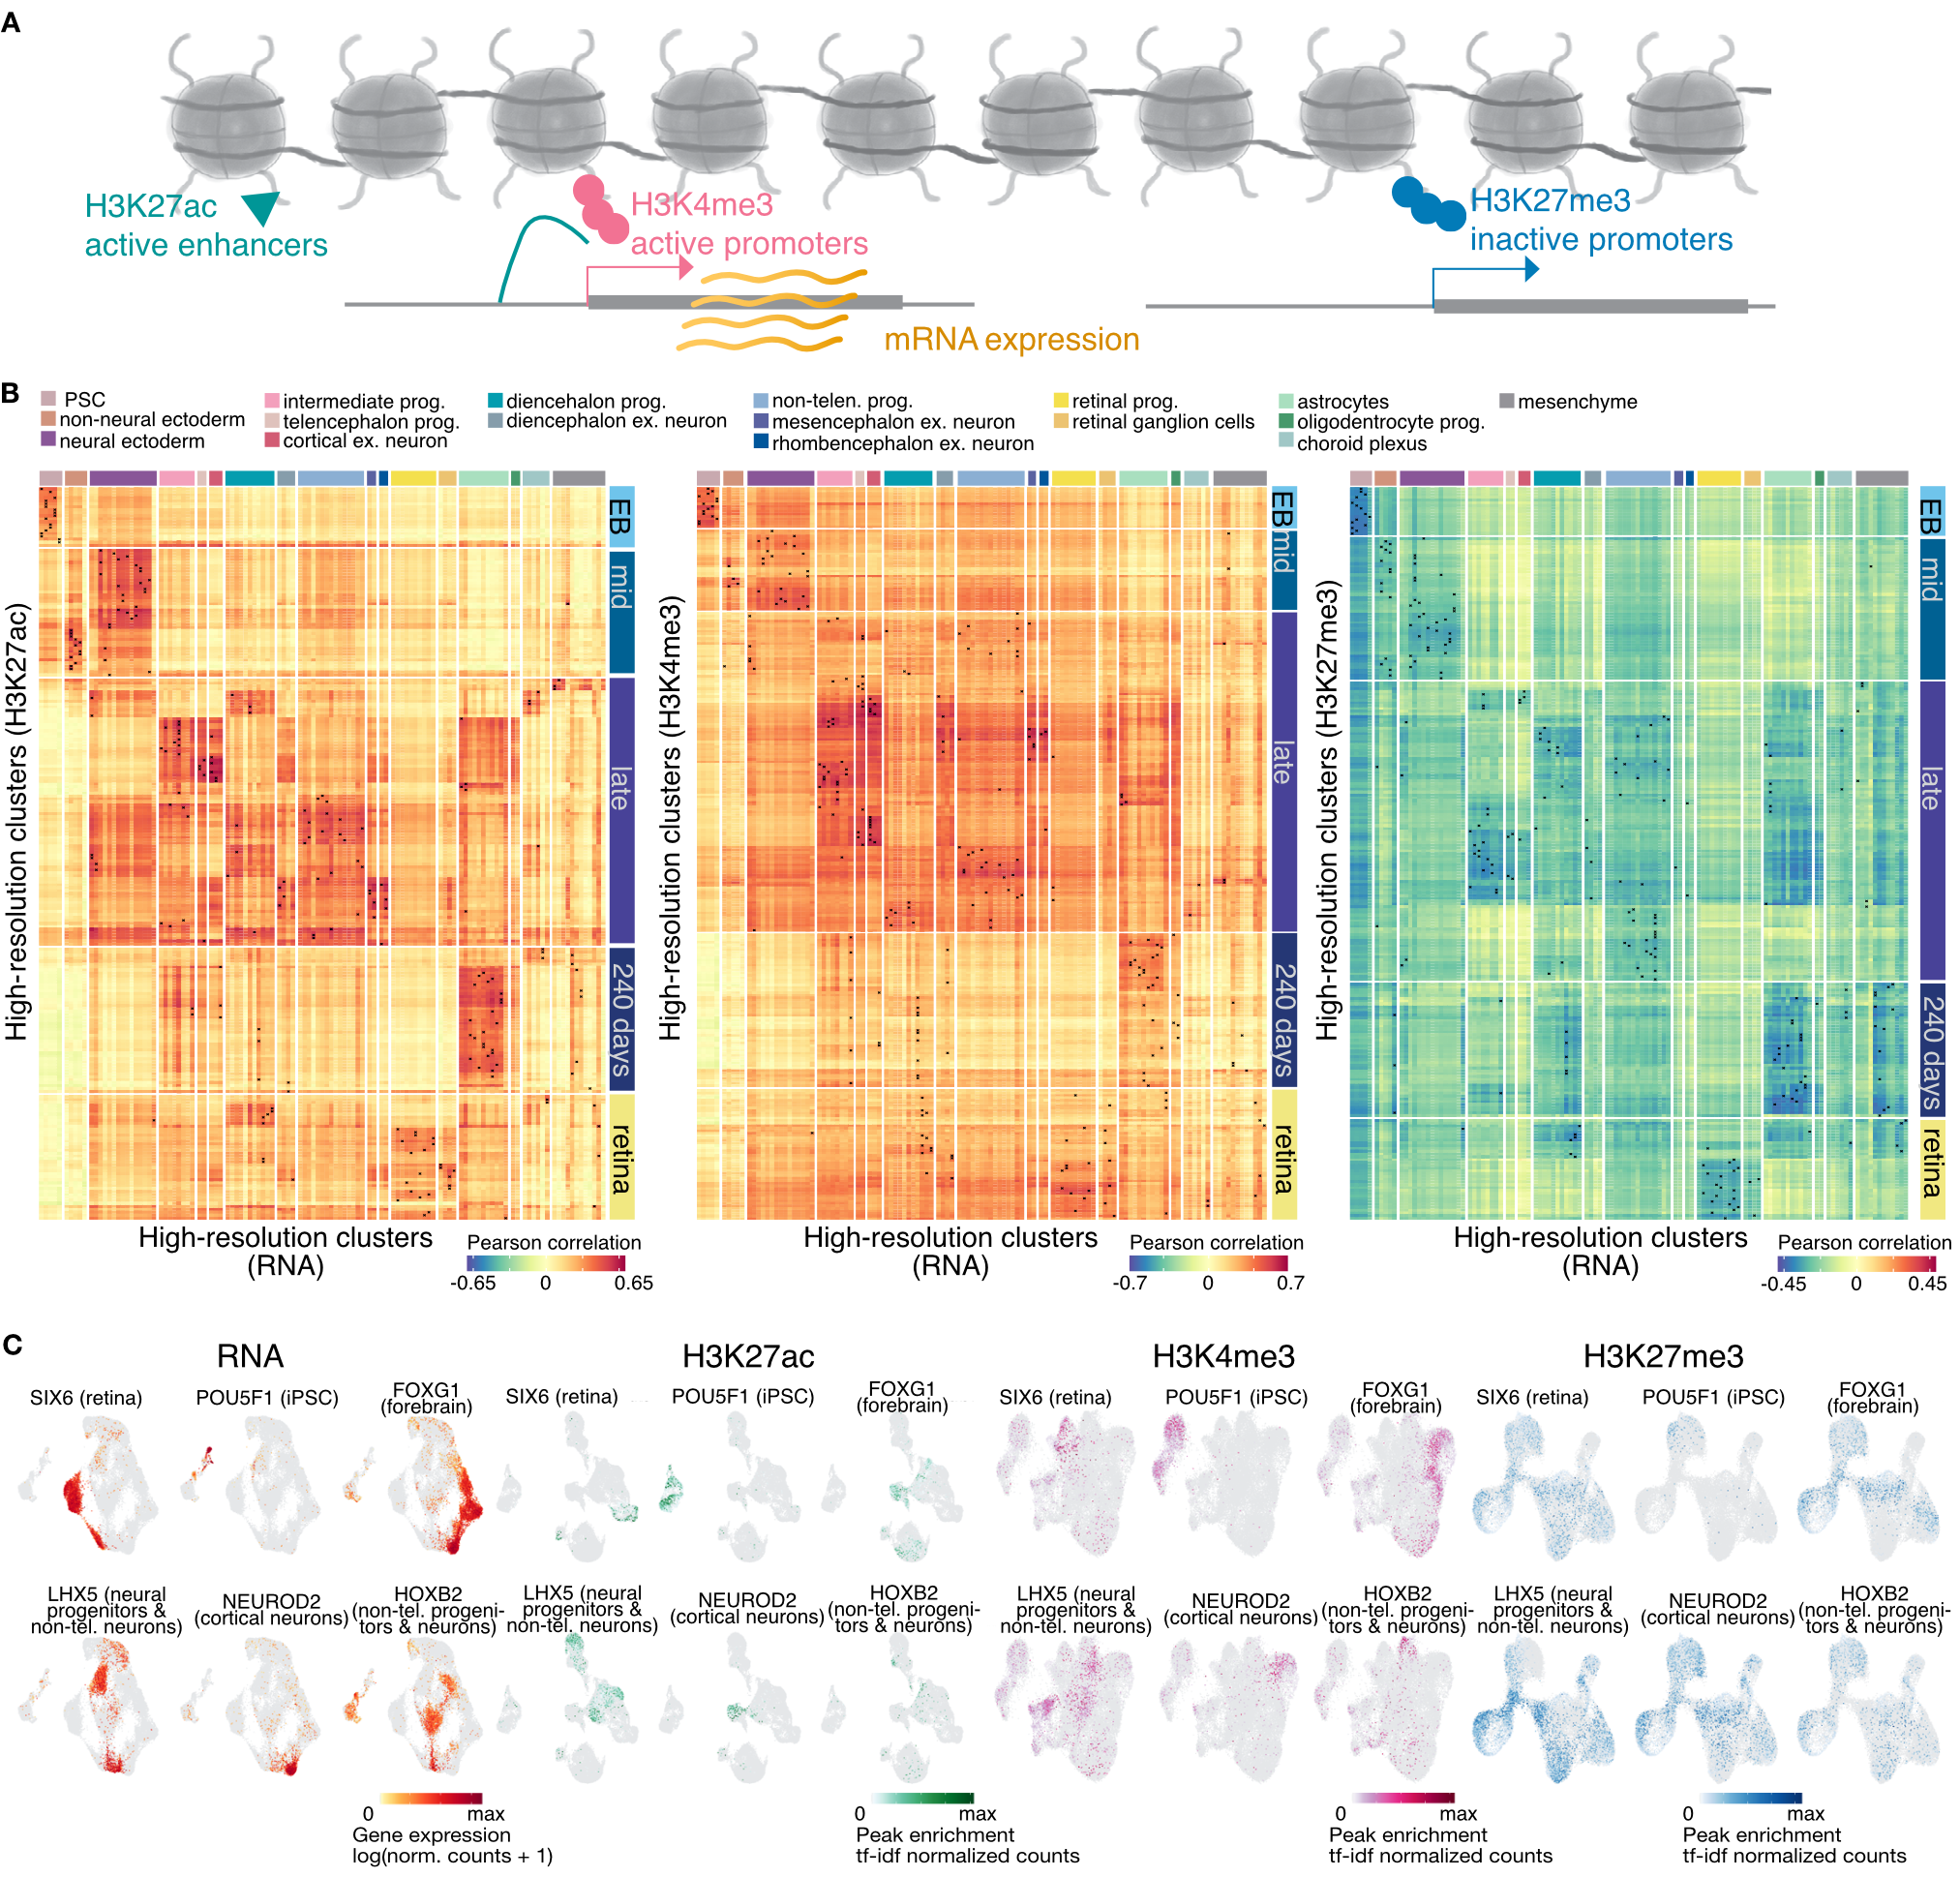
\includegraphics[width=\textwidth]{figures/cnt/Figure_S2}
    \label{fig:regS2}
    \caption{\textbf{Multi-modal matching between high-resolution clusters.}
    (A) Schematic of profiled modalities. H3K27ac marks active promoters and enhancers, H3K4me3 marks active promoters. H3K27me3 marks repressed regions with inactive promoters. (B) Heatmaps showing correlation and matching of high-resolution clusters across modalities. Matched clusters are indicated with a cross. (C) UMAP representation of all modalities in the developmental time course colored by expression (log(transcript counts per 10k + 1); in case of RNA-seq) and gene activity (log(fragment counts per 10k + 1); in case of Cut\&Tag) of genes marking celltypes.}
\end{figure}


\begin{figure}[h!]
    \centering
	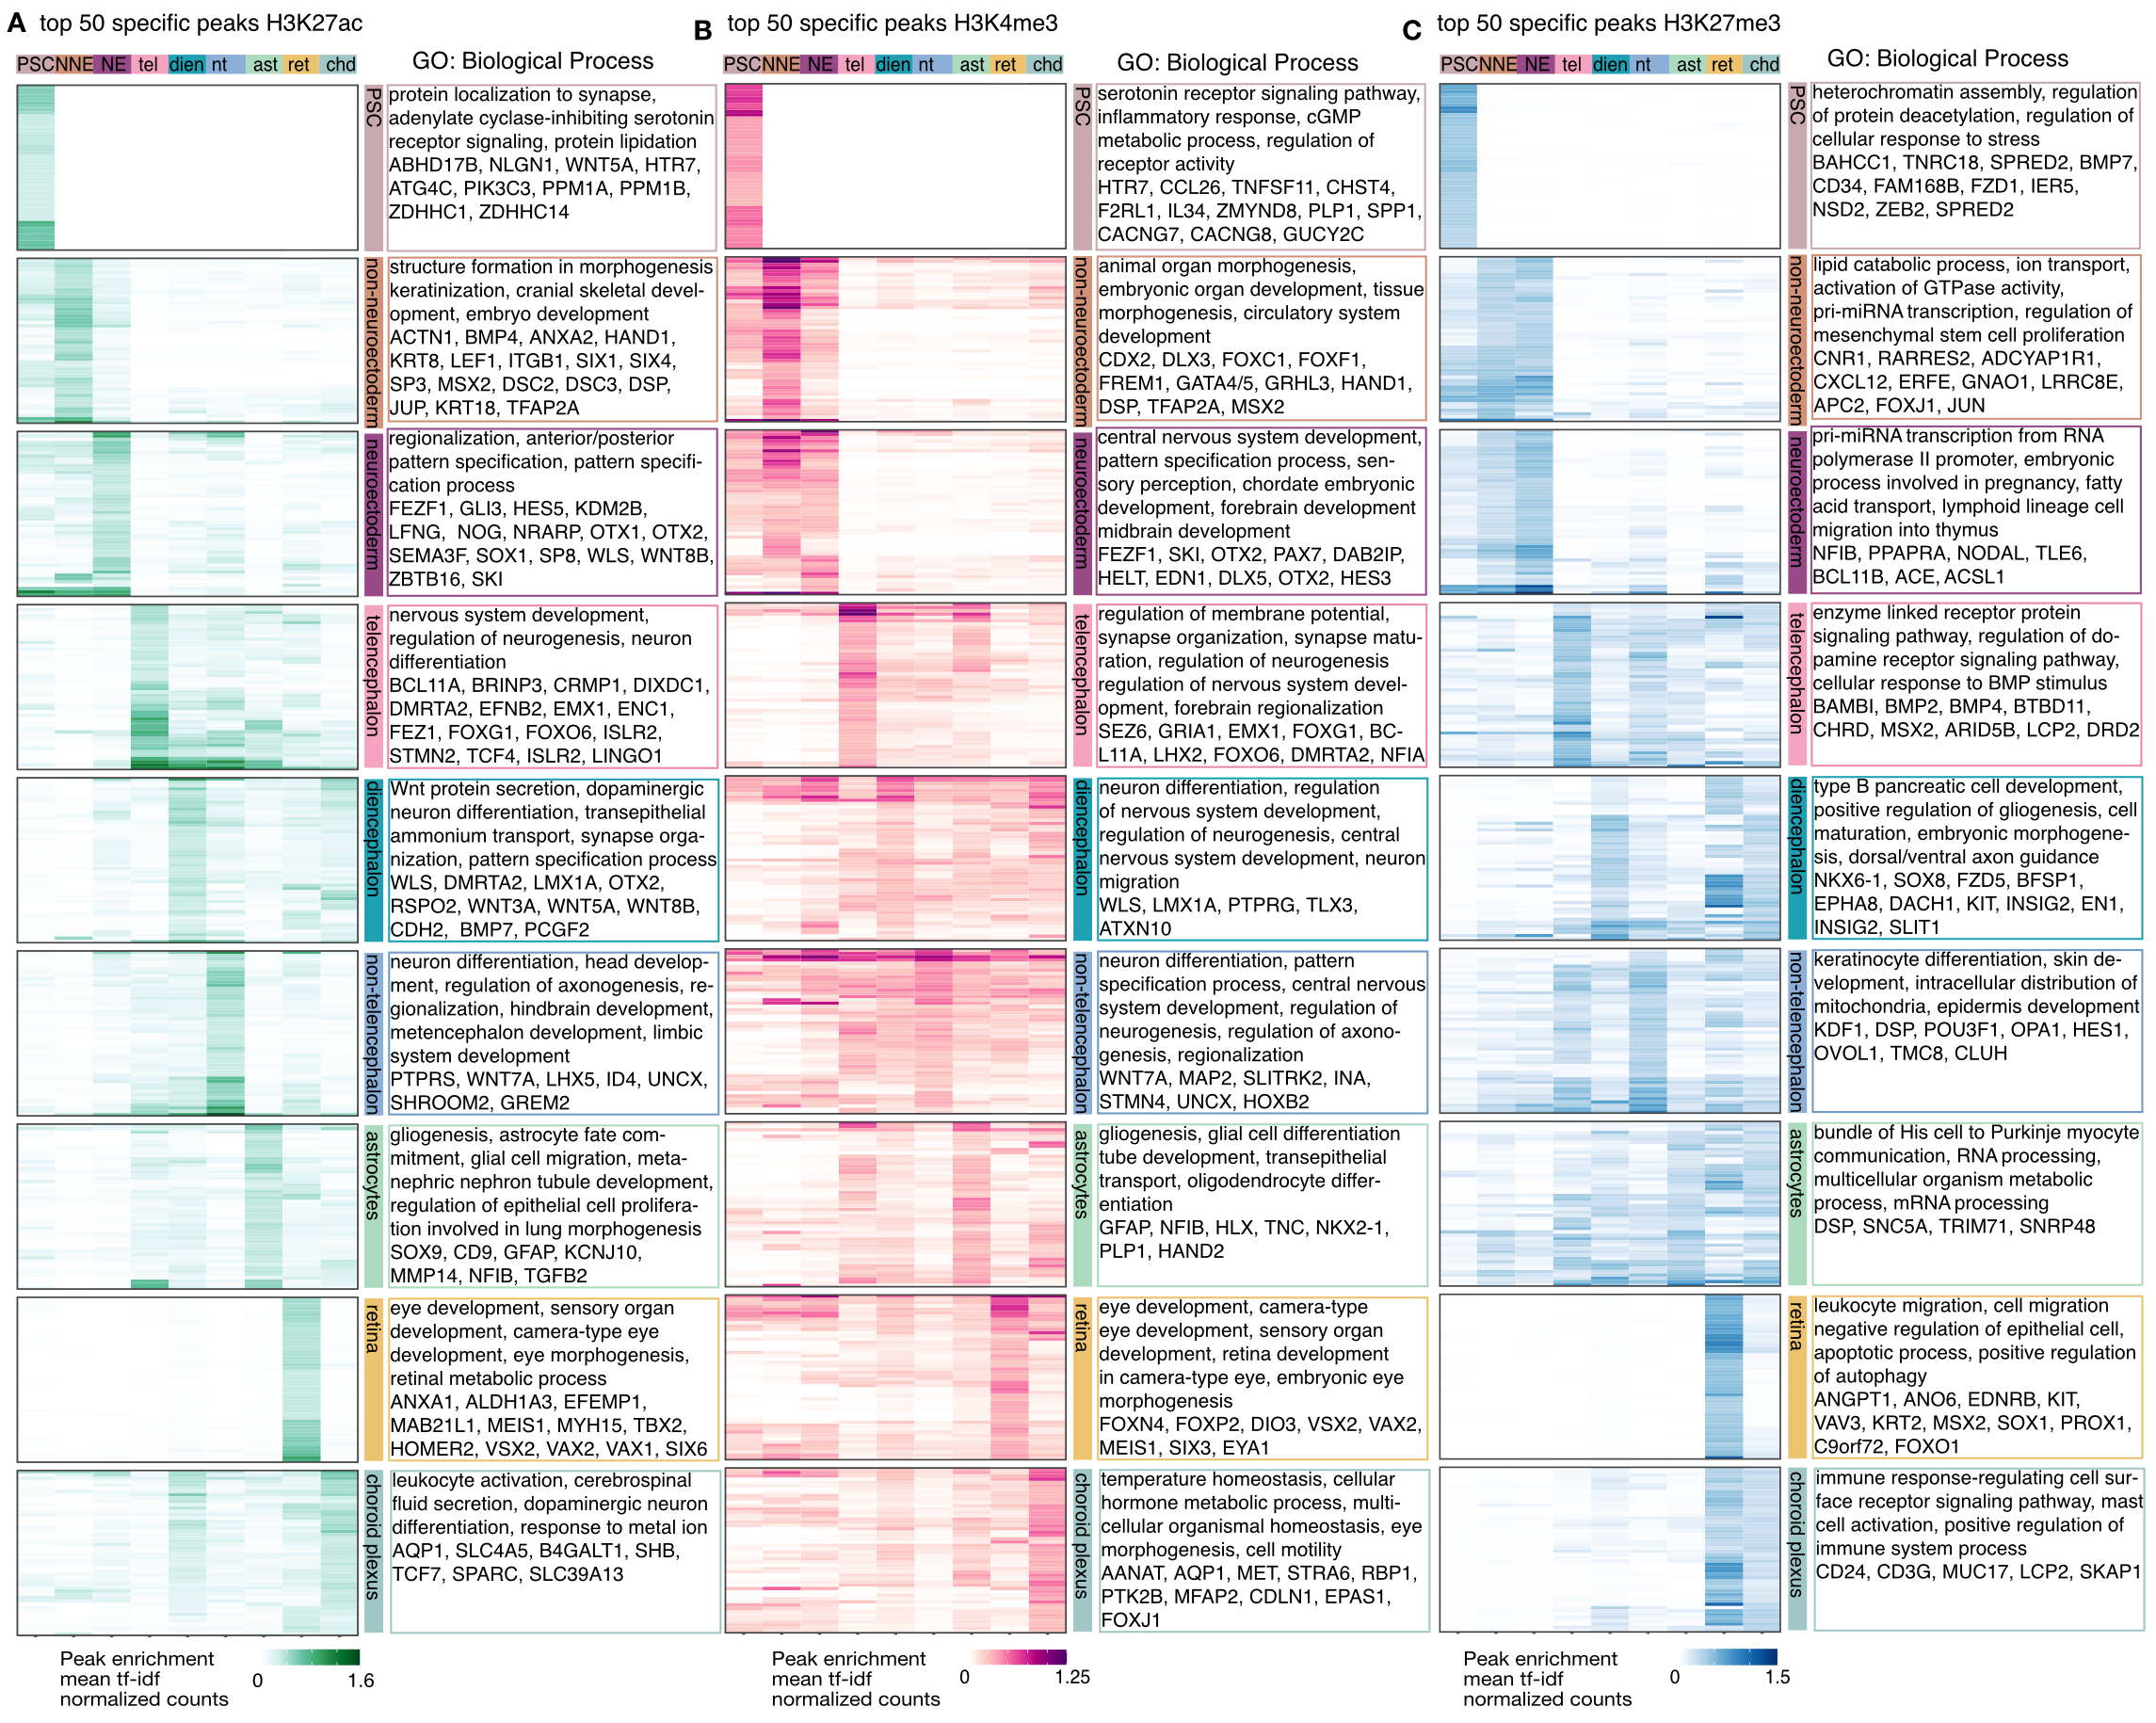
\includegraphics[width=\textwidth]{figures/cnt/Figure_S3}
    \label{fig:regS3}
    \caption{\textbf{Cell type- and region-specific chromatin modification peaks.}
    (A, B, C) Heatmaps showing tf-idf normalized peak counts of state- and region-specific peaks for (A) H3K27ac, (B) H3K4me3 and (C) H3K27me3. Selected genes in proximity to these peaks and representative GO Biological Process terms are indicated on the right.}
\end{figure}

